\chapter{Frontend Implementation and User Flows}
\label{chap:frontend_implementation}

\section{Introduction}
\label{sec:ch4_introduction}

The previous chapter studied the backend domain model and the business modules that support Supply Chain Finance operations. This chapter moves to the frontend layer, where those domain concepts become usable screens, forms, tables, wizards, modals, and navigation flows. A financing platform may have a strong backend model, but users experience it through interaction: selecting a program, uploading invoices, submitting a request, reviewing validation errors, or opening a transaction detail view.

The frontend of the SCF platform is implemented as a React single-page application built with Vite and TypeScript. It relies on React Router for navigation, React Query for server-state handling, Axios for API calls, Keycloak for authentication, and a UI component base built around shadcn/ui and Radix UI. The implementation is organized around feature modules such as master setup, counterparty onboarding, invoice upload, finance disbursement, early payment, transaction inquiry, document inquiry, and foundational data management.

\section{Application Architecture and Navigation}
\label{sec:application_navigation}

\subsection{Application Entry Point and Route Structure}
\label{subsec:app_entry_routes}

The application starts from \texttt{App.tsx}. This file assembles the global providers and route structure. The available routes include \texttt{/auth}, the main protected route \texttt{/}, and \texttt{/specification-document}. The application is wrapped with \texttt{KeycloakAuthProvider}, \texttt{QueryClientProvider}, \texttt{Toaster}, and \texttt{TooltipProvider}. This arrangement gives the interface access to authentication state, server-state caching, user feedback, and tooltip behavior from the top of the component tree.

The main route is protected by \texttt{AuthGuard}. If authentication is still loading, the guard displays a loading state. If the user is not authenticated, it redirects to the authentication page. If the user is authenticated, it allows the main interface to render.

\subsection{Role-Based Sidebar and View Adaptation}
\label{subsec:role_sidebar}

The role system is one of the frontend's central mechanisms. The decoded Keycloak token contains realm roles. The helper \texttt{businessViewFromRoles.ts} reads these roles and derives one of three business views: \texttt{BANK}, \texttt{ANCHOR}, or \texttt{COUNTERPARTY}. The \texttt{useBusinessView} hook exposes the resulting view and convenience flags such as \texttt{isBank}, \texttt{isAnchor}, and \texttt{isCounterparty}.

Figure~\ref{fig:ch4_navigation_role_flow} shows how routing, authentication, and business-view adaptation fit together.

\begin{figure}[H]
    \centering
    
\includegraphics[width=\textwidth, keepaspectratio]{images/ch4_navigation_role_flow.png}
    \caption{Frontend routing and role-based navigation}
    \label{fig:ch4_navigation_role_flow}
\end{figure}

The \texttt{AppSidebar} filters menu items according to the business view. Bank users see the broadest set of modules, including master setup, transaction inquiry, document inquiry, invoice management, early payment, and finance disbursement. Anchor users see a narrower set focused on their own operational activities, such as invoice upload, manual invoice entry, transaction inquiry, and early payment. Counterparty users receive an even more focused view, centered on their own invoices, transactions, and payment requests.

\begin{figure}[H]
    \centering
    
\includegraphics[width=\textwidth, keepaspectratio]{images/ch4_use_case_back_office.png}
    \caption{Back-office use cases for bank maker and checker roles}
    \label{fig:ch4_use_case_back_office}
\end{figure}

\begin{figure}[H]
    \centering
    
\includegraphics[width=\textwidth, keepaspectratio]{images/ch4_use_case_middle_office.png}
    \caption{Middle-office use cases for monitoring and follow-up}
    \label{fig:ch4_use_case_middle_office}
\end{figure}

\begin{figure}[H]
    \centering
    
\includegraphics[width=\textwidth, keepaspectratio]{images/ch4_use_case_front_office.png}
    \caption{Front-office use cases for buyer and supplier actions}
    \label{fig:ch4_use_case_front_office}
\end{figure}

\begin{figure}[H]
    \centering
    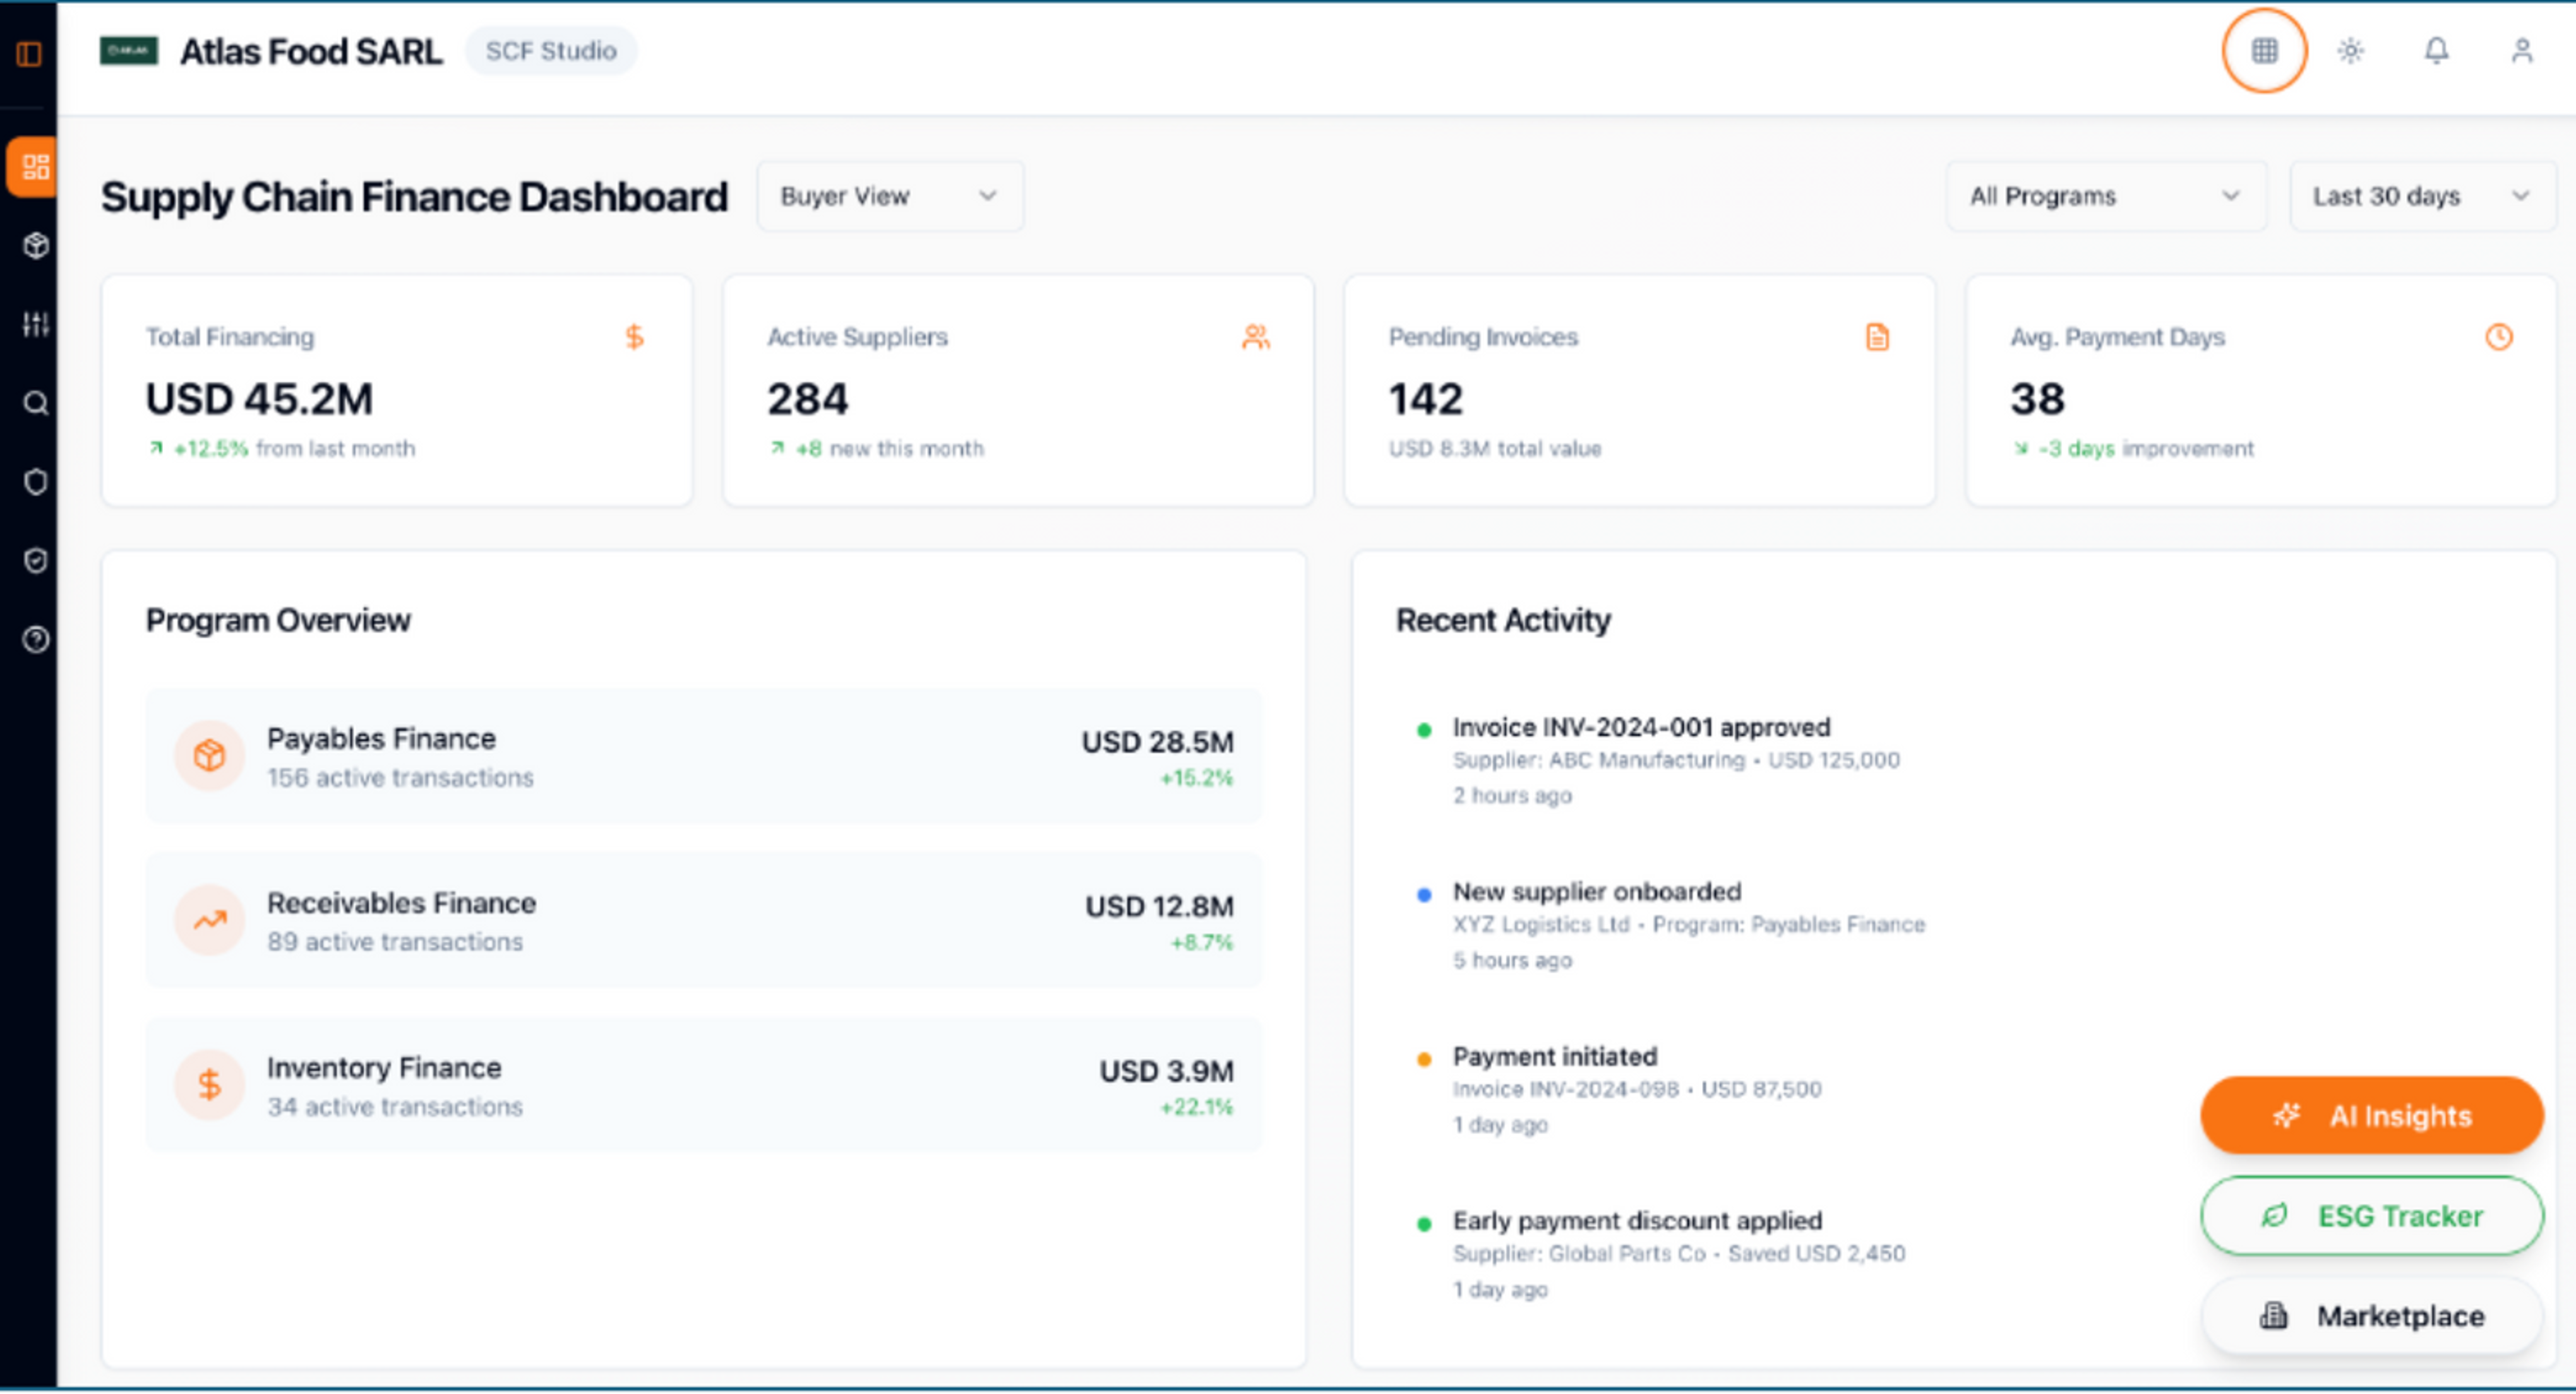
\includegraphics[width=\textwidth, keepaspectratio]{images/platform_scf_dashboard_light.png}
    \caption{SCF dashboard in light mode with business-view filtering}
    \label{fig:ch4_scf_dashboard_light}
\end{figure}

\begin{figure}[H]
    \centering
    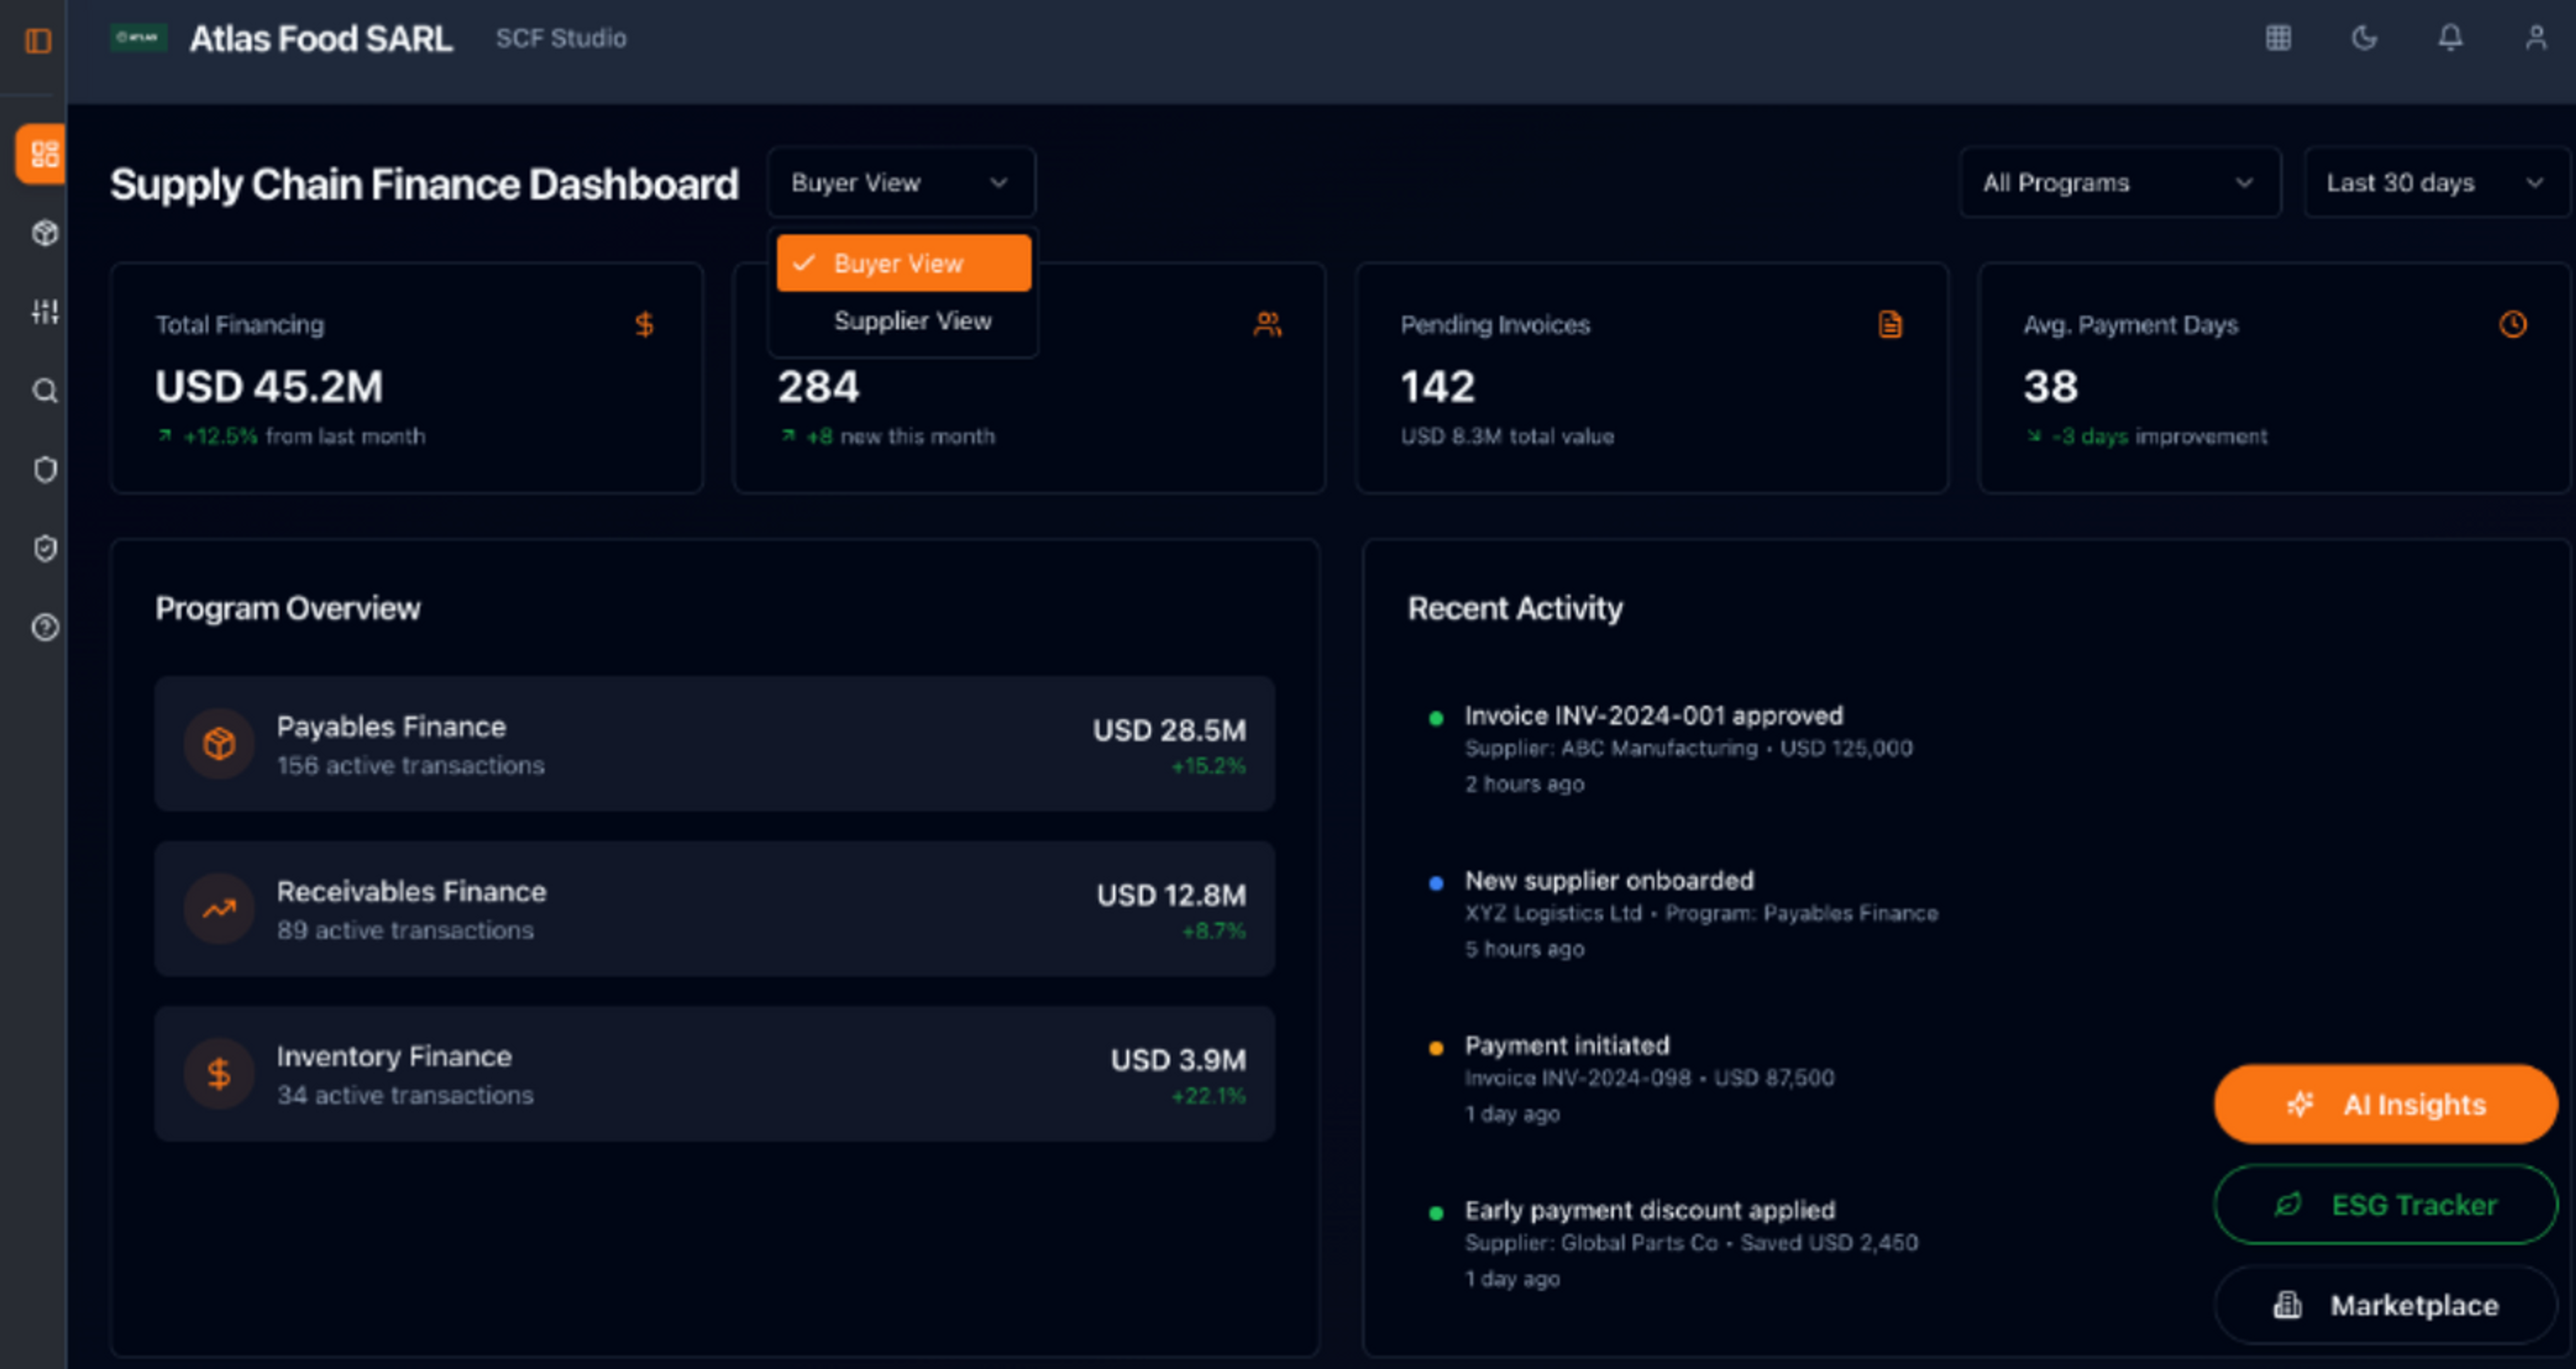
\includegraphics[width=\textwidth, keepaspectratio]{images/platform_scf_dashboard_dark.png}
    \caption{SCF dashboard in dark mode with buyer and supplier view selector}
    \label{fig:ch4_scf_dashboard_dark}
\end{figure}

\subsection{\texttt{Index.tsx} and Module Selection}
\label{subsec:index_module_selection}

The \texttt{Index.tsx} page renders the sidebar and a content area driven by a \texttt{selectedModule} state. This state decides which functional component is displayed: dashboard, master setup, transaction inquiry, document inquiry, invoice upload, invoice form, finance disbursement, early payment, or notifications. This approach keeps the primary workspace inside a single routed page while still allowing the user to move between modules.

The design is pragmatic. It avoids turning every module switch into a full route transition, while the application still keeps authentication and global providers outside the page. For an operational banking interface, this feels natural: the user remains inside a controlled workspace and changes the working panel from the sidebar.

\begin{figure}[H]
    \centering
    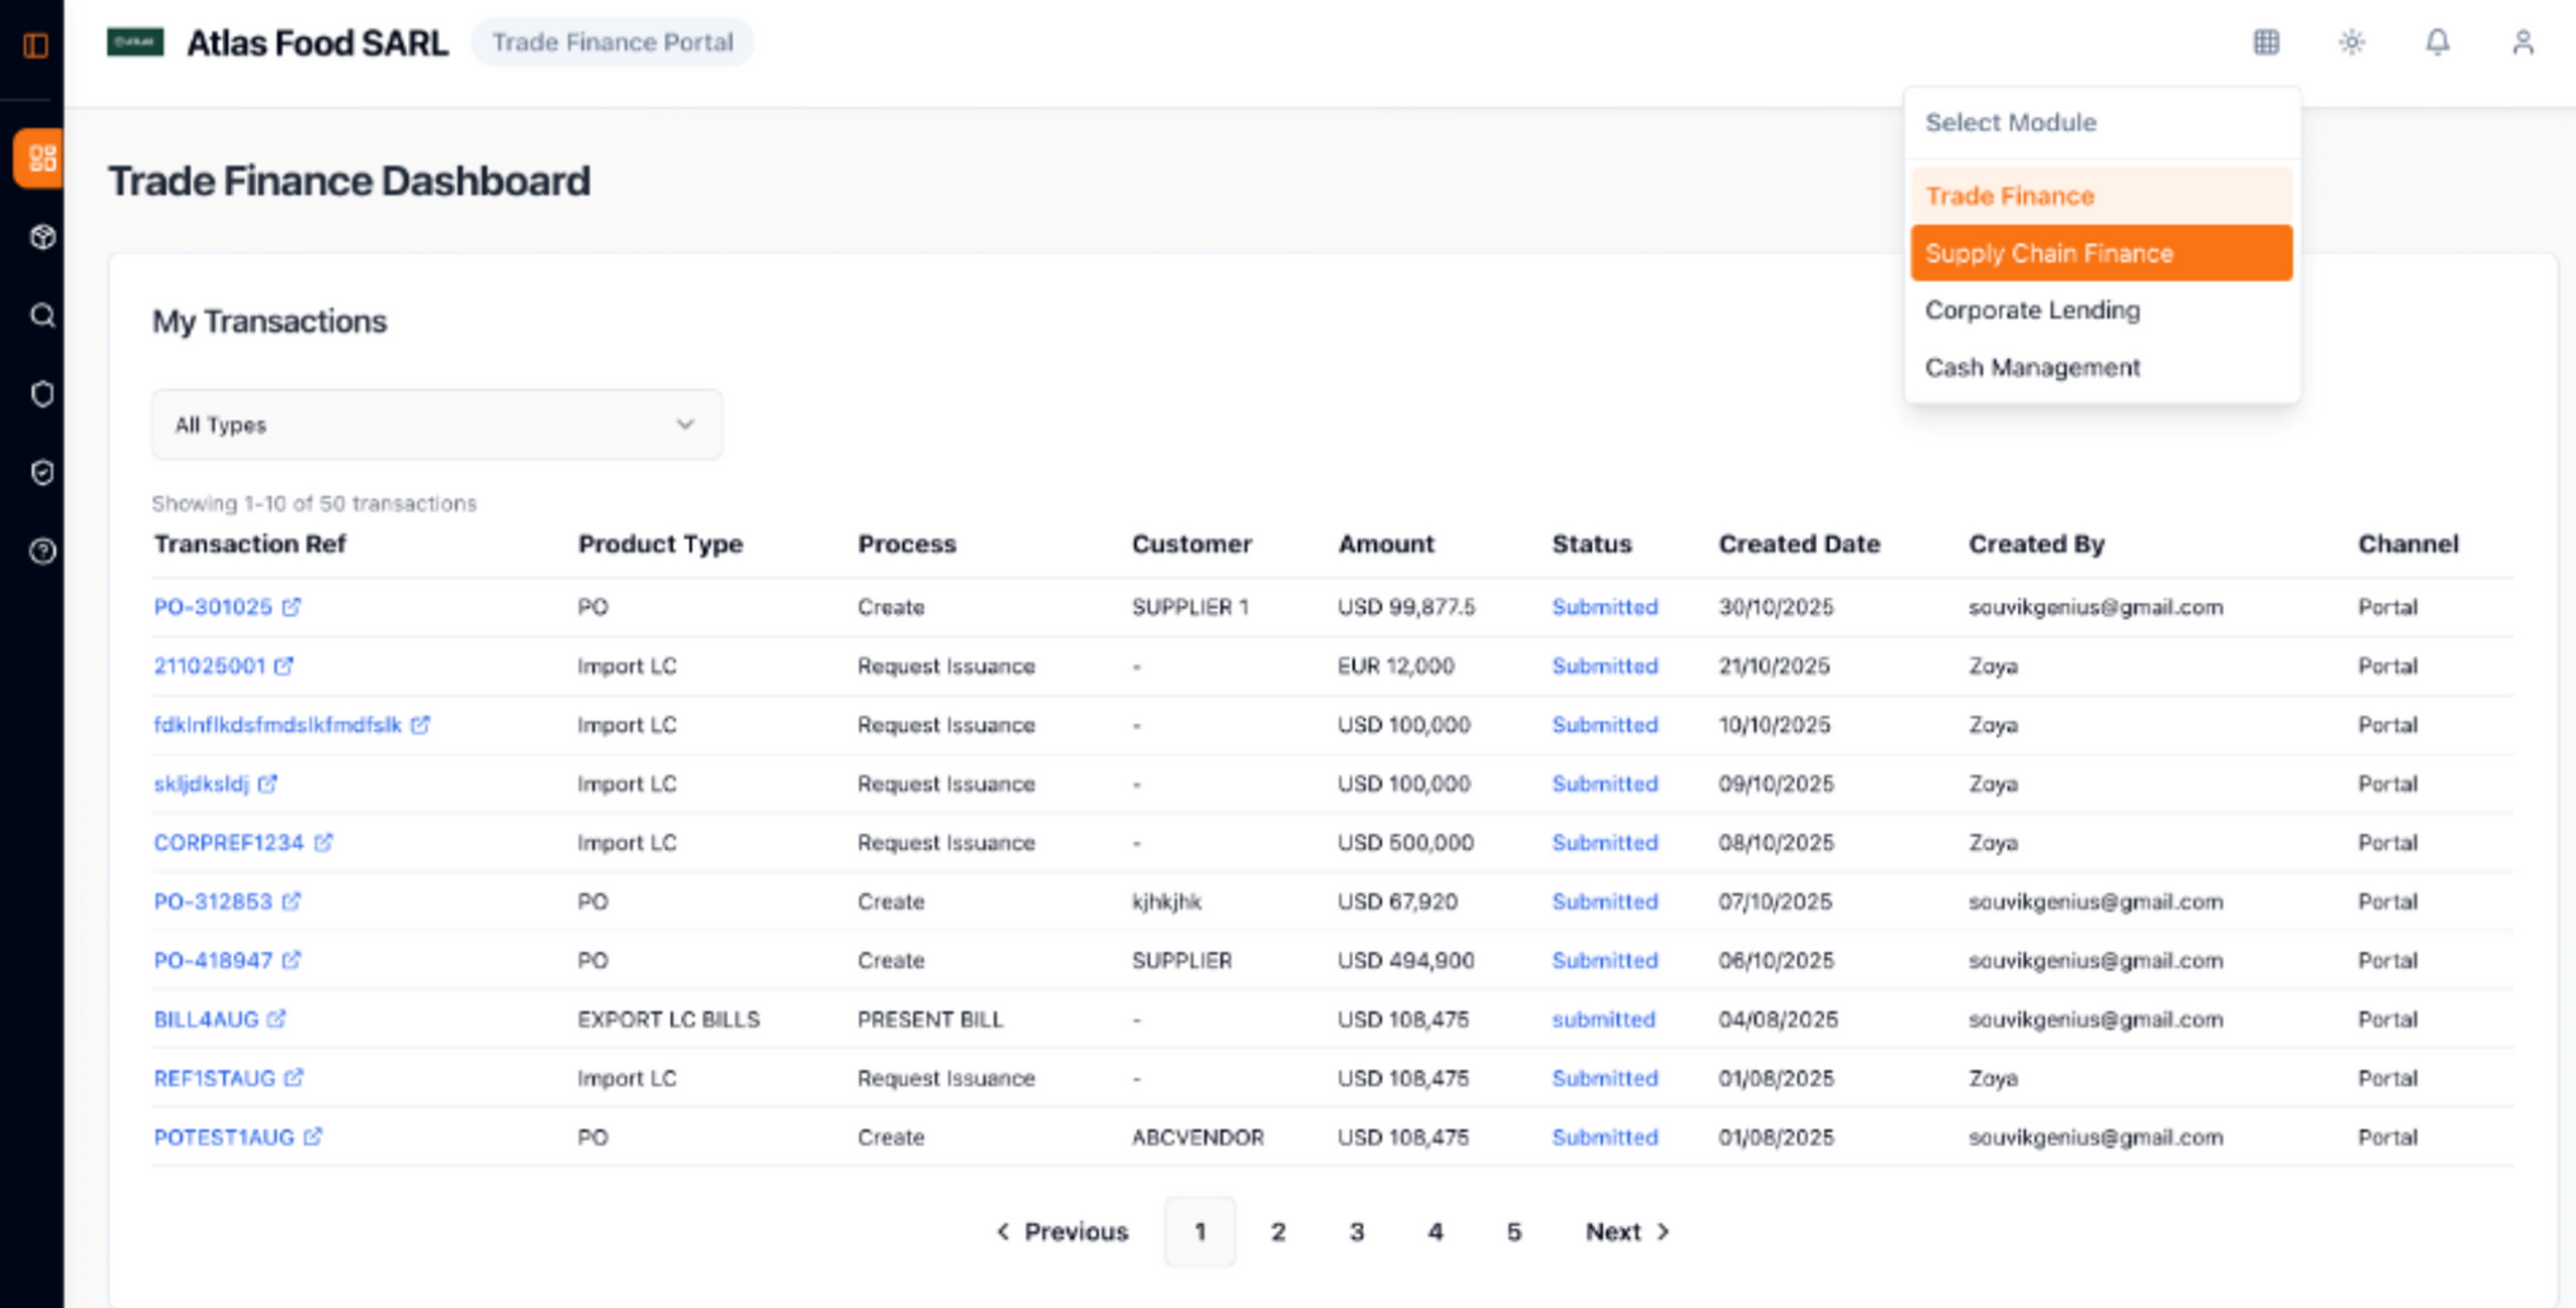
\includegraphics[width=\textwidth, keepaspectratio]{images/platform_scf_module_switch.png}
    \caption{Module switch between Trade Finance and Supply Chain Finance}
    \label{fig:ch4_module_switch}
\end{figure}

\section{Master Setup Module}
\label{sec:master_setup_module}

\subsection{Tab Structure and Role-Gated Access}
\label{subsec:master_setup_tabs}

\texttt{SCFMasterSetup} acts as a container for several administrative and configuration modules. Its tabs include product suite, program configuration, counterparty onboarding, foundational data, and control centre features. Access to these tabs is role-gated, which prevents users outside the bank view from reaching administrative functions that do not belong to their business position.

\begin{figure}[H]
    \centering
    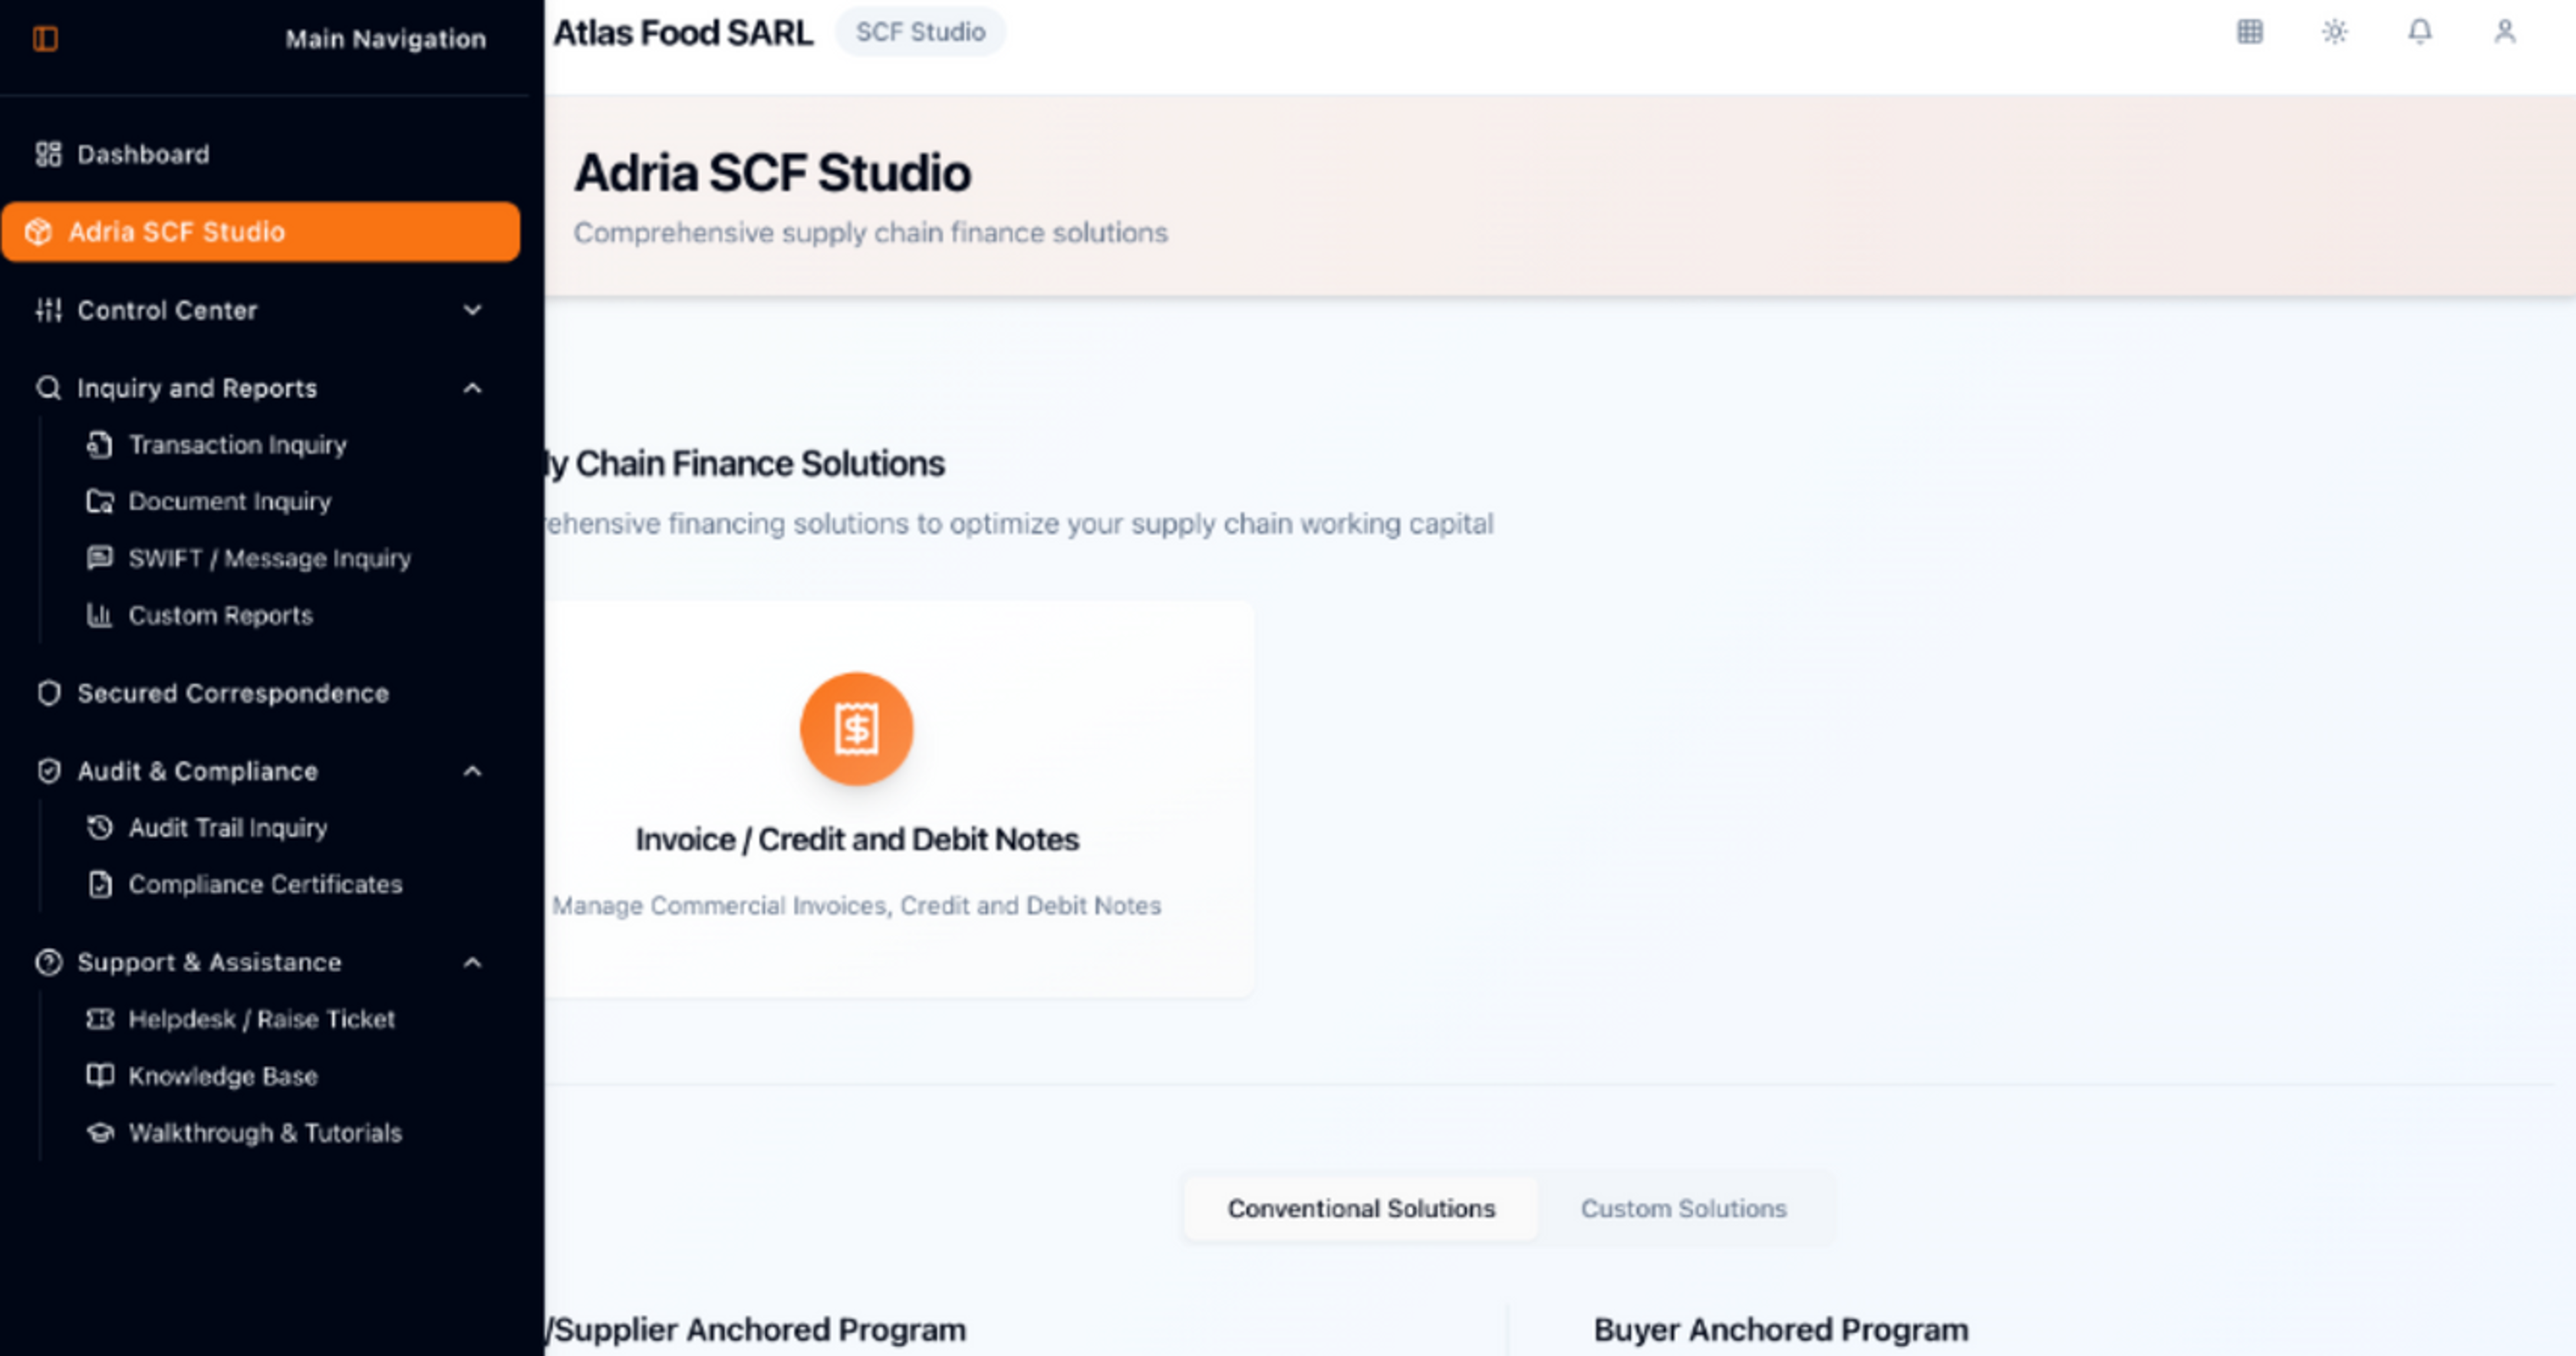
\includegraphics[width=\textwidth, keepaspectratio]{images/platform_navigation_menu.png}
    \caption{Navigation menu exposing SCF Studio and inquiry modules}
    \label{fig:ch4_navigation_menu_screenshot}
\end{figure}

\subsection{Product Suite and Program Configuration}
\label{subsec:product_program_ui}

The product suite exposes product definition management through \texttt{SCFProductSuite}, \texttt{SCFProductDefinition}, and product-related components such as \texttt{ProductSolutionToggle}. This interface allows the bank side to view, create, or edit product templates according to the supported SCF product families.

\begin{figure}[H]
    \centering
    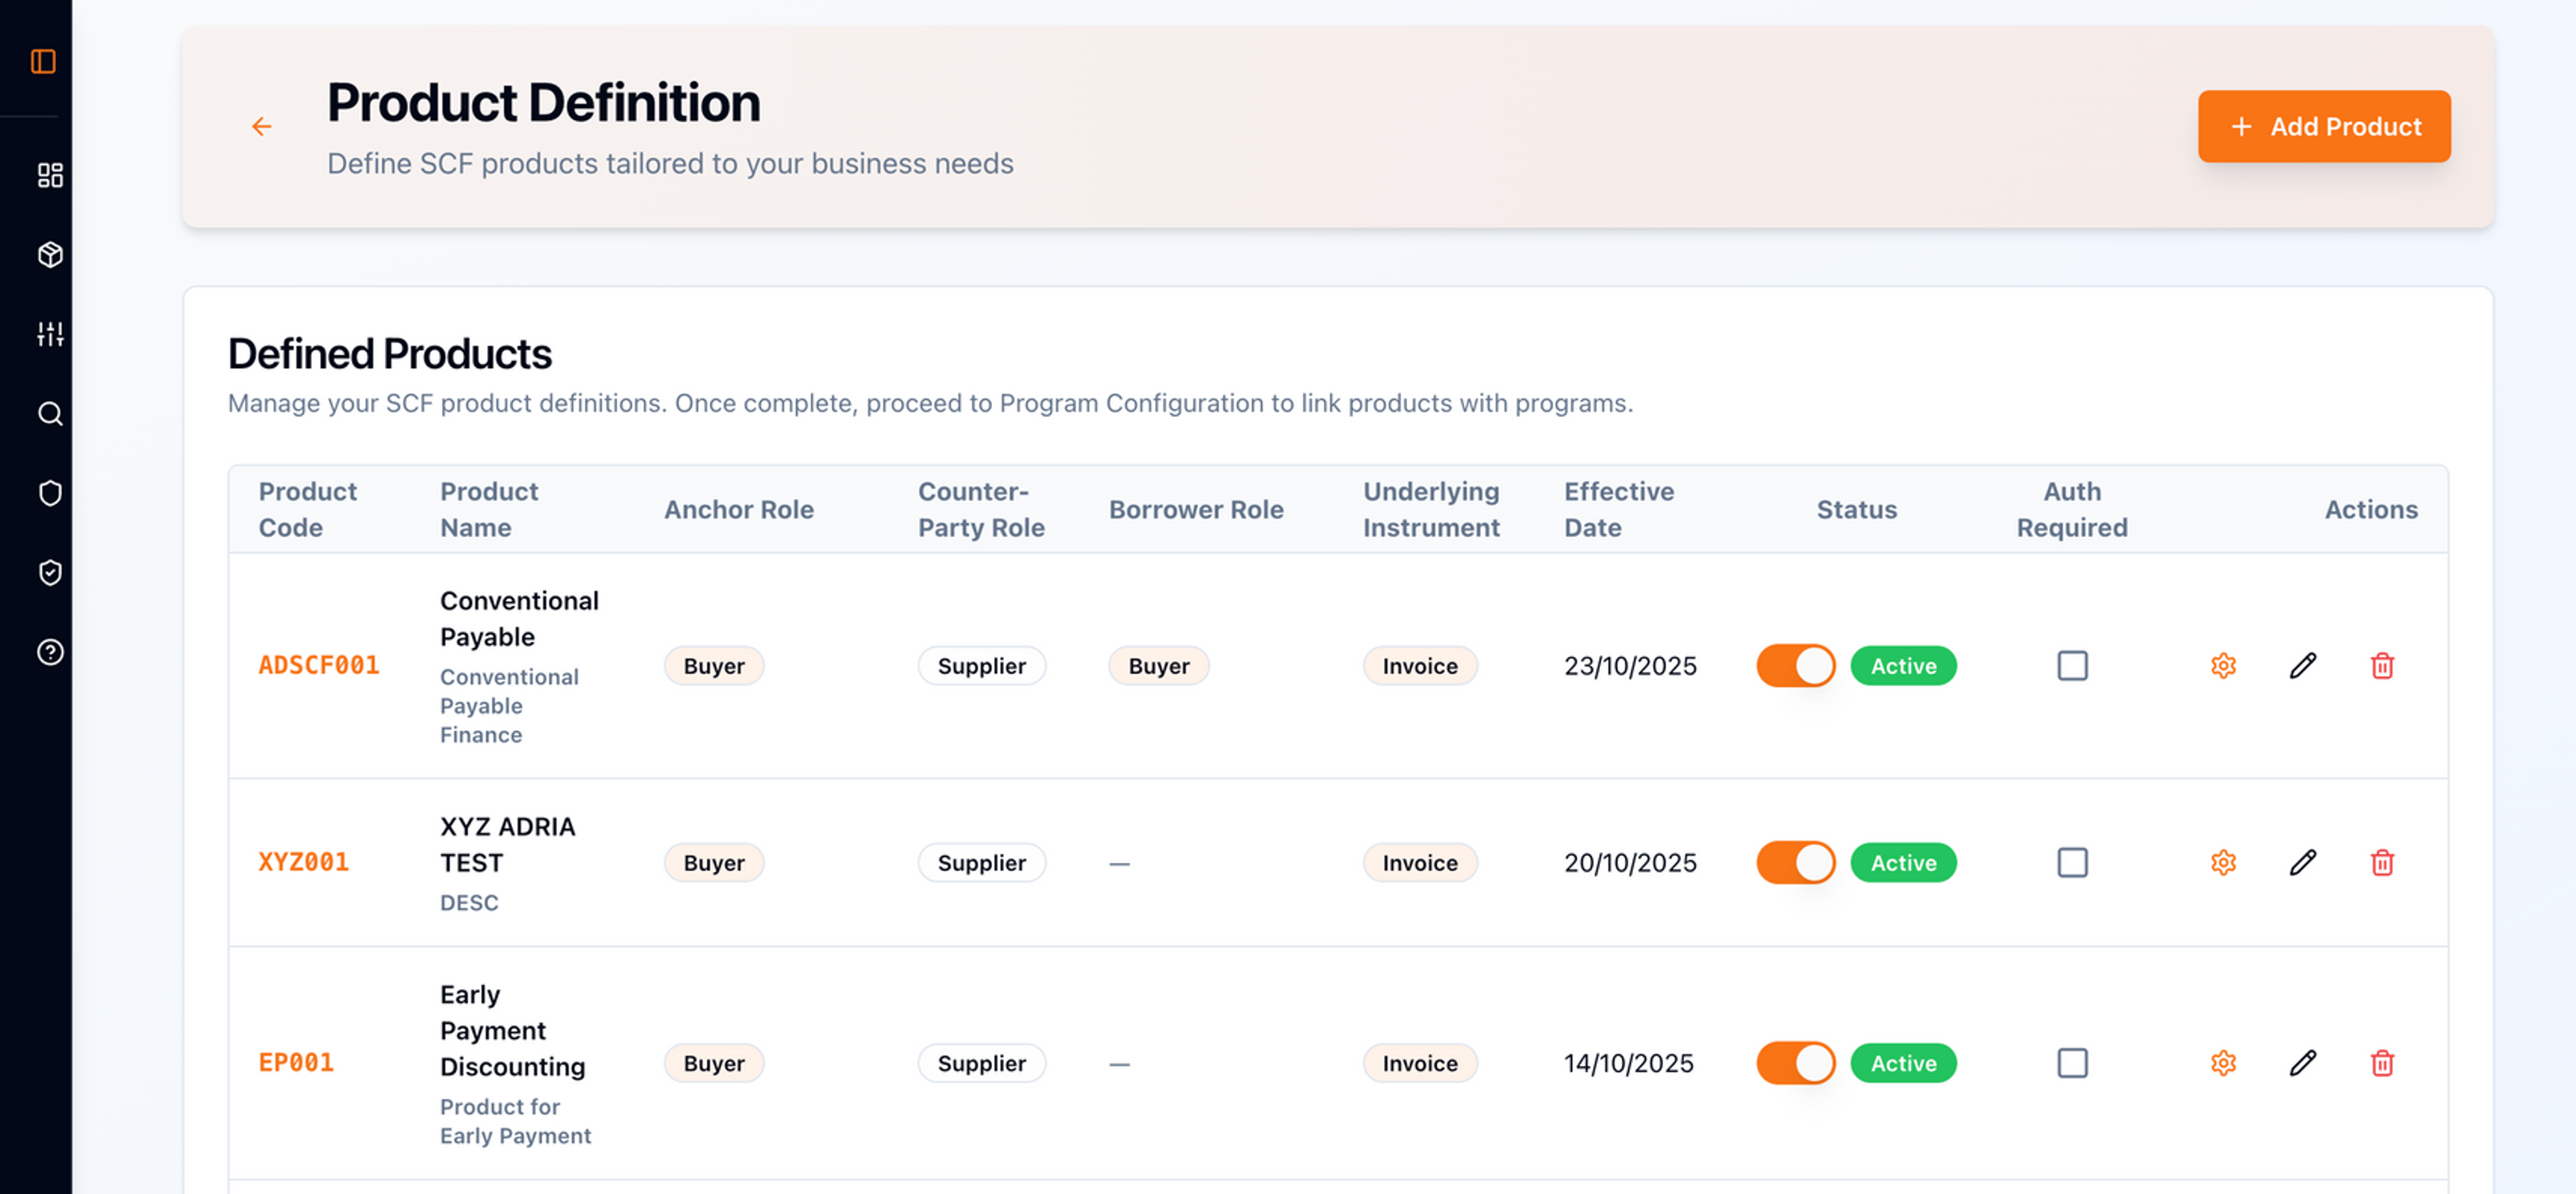
\includegraphics[width=\textwidth, keepaspectratio]{images/platform_product_configurator.png}
    \caption{Product definition list in the SCF product configurator}
    \label{fig:ch4_product_configurator}
\end{figure}

\begin{figure}[H]
    \centering
    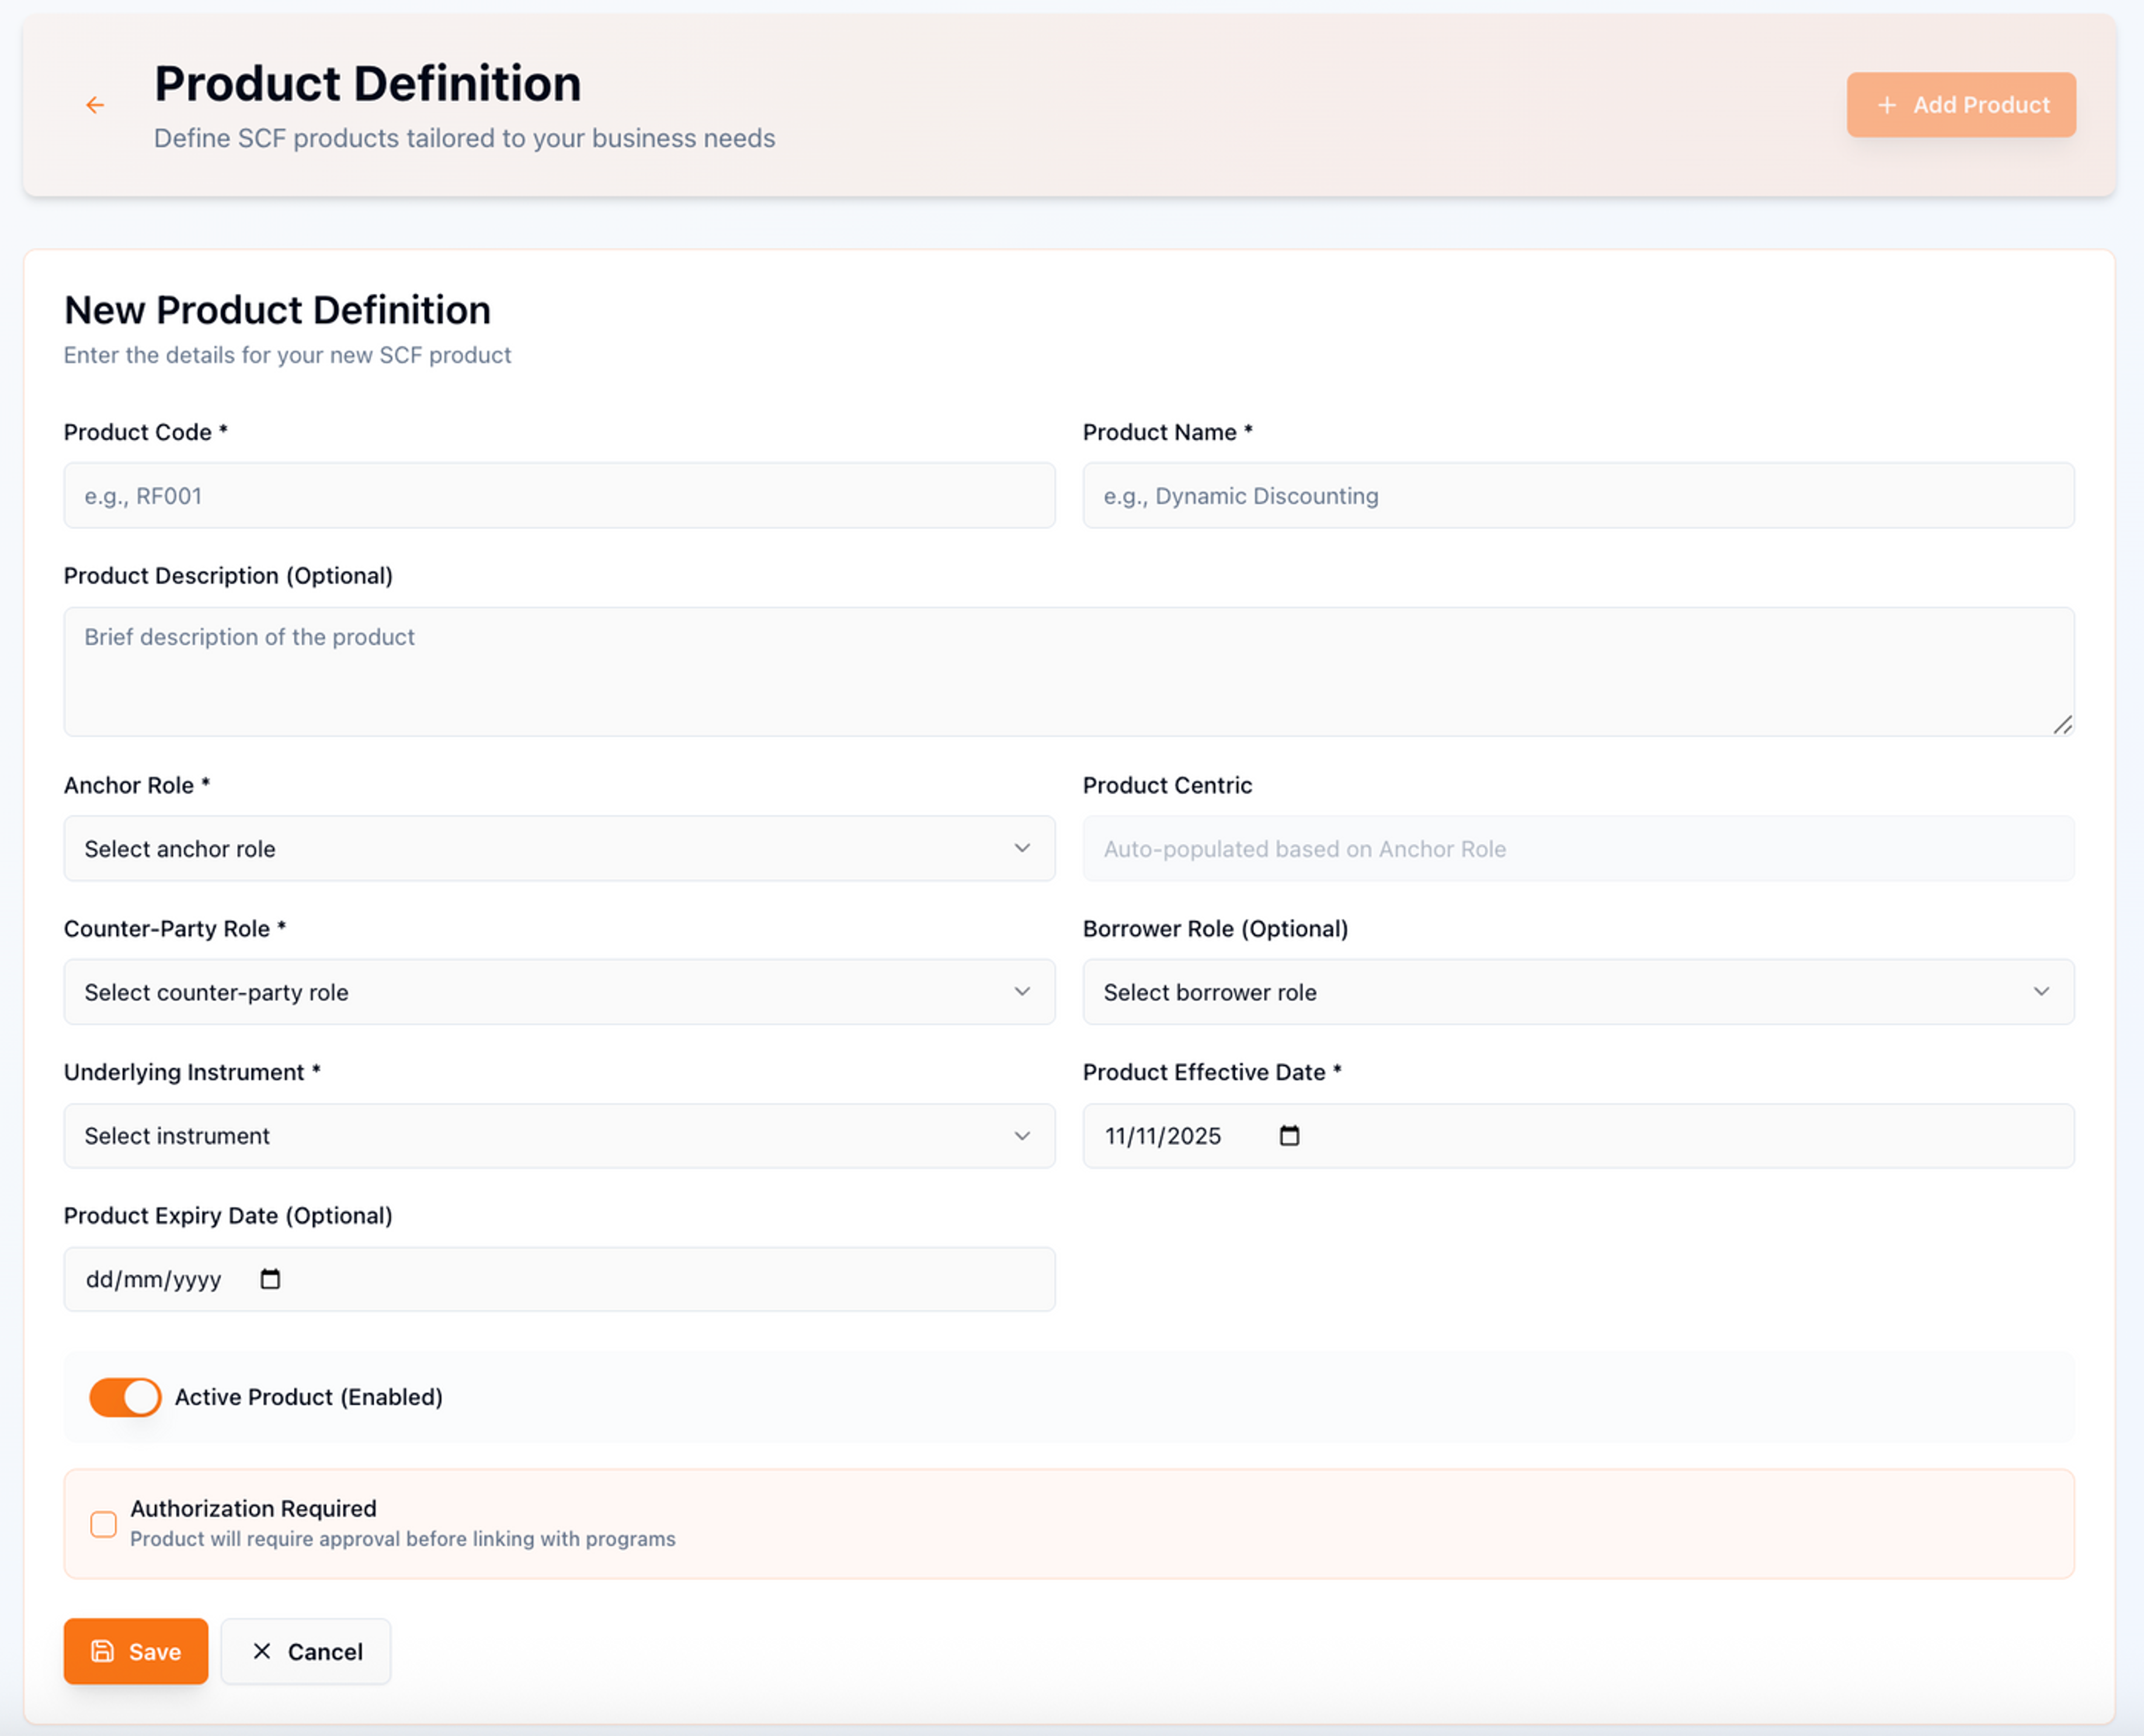
\includegraphics[width=\textwidth, keepaspectratio]{images/platform_product_creation_form.png}
    \caption{Product definition creation form}
    \label{fig:ch4_product_creation_form}
\end{figure}

Program configuration is handled by \texttt{SCFProgramConfiguration} and \texttt{ProgramFormDialog}. The dialog is structured as a multi-step configuration process: \texttt{GeneralPartyPane}, \texttt{FeeCataloguePane}, and \texttt{DisbursementRepaymentPane}. The \texttt{useProgramForm} hook centralizes the form state and helps keep the wizard logic outside individual panes.

\begin{figure}[H]
    \centering
    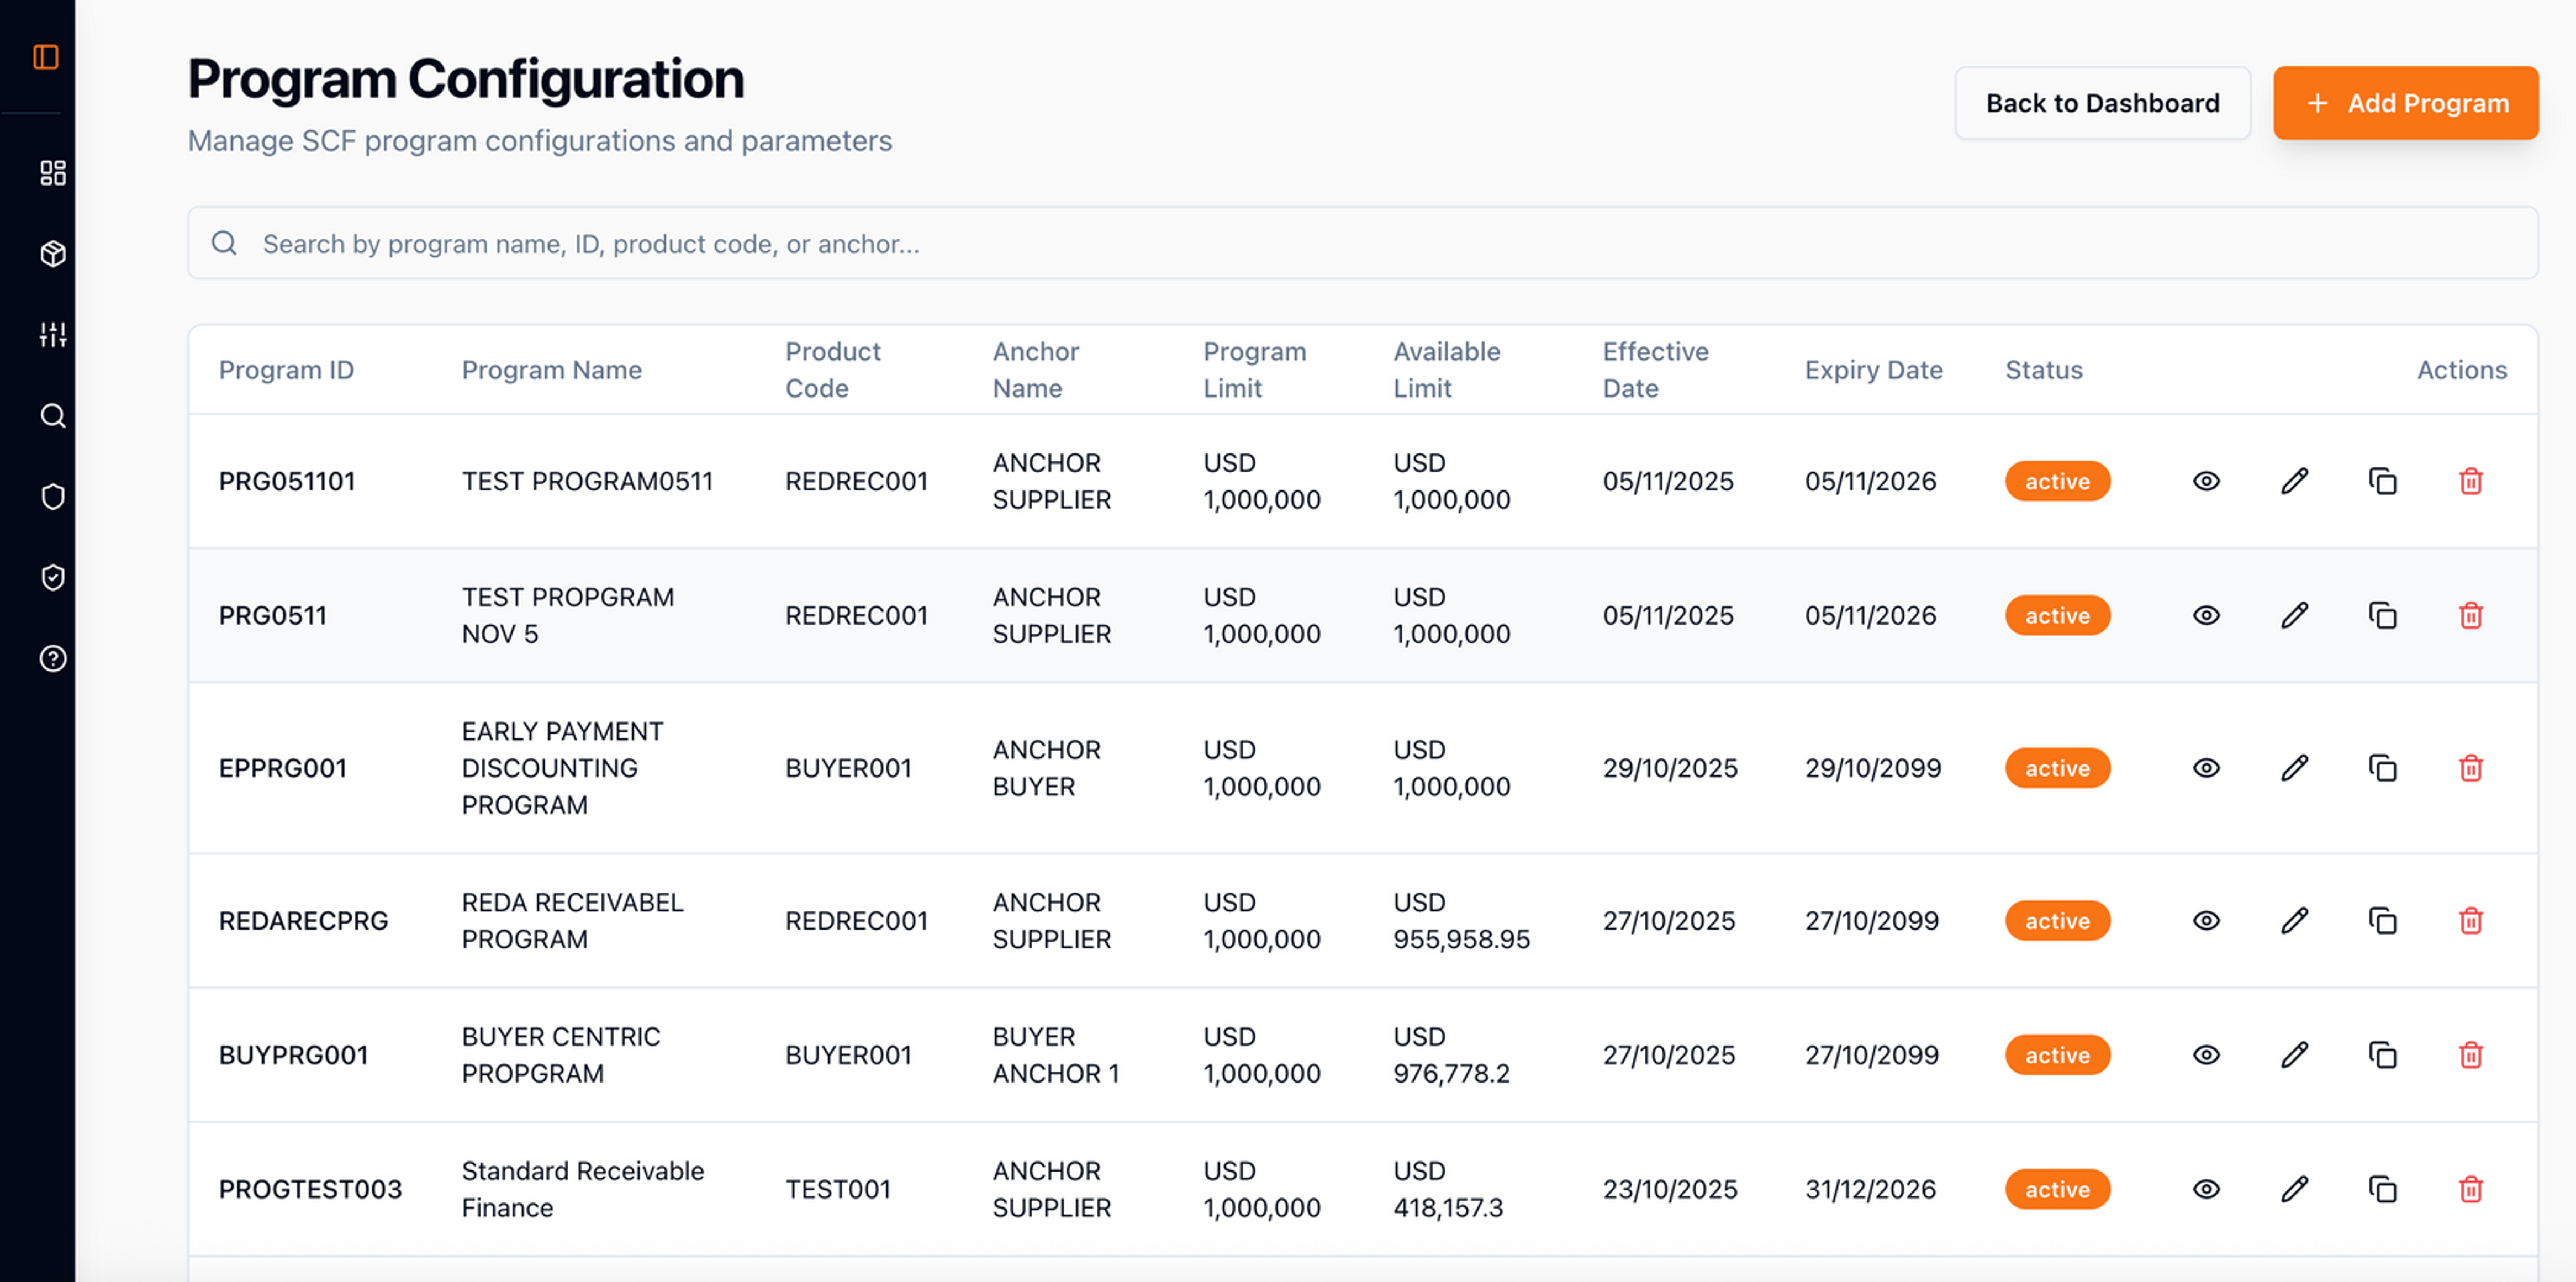
\includegraphics[width=\textwidth, keepaspectratio]{images/platform_program_configurator.png}
    \caption{Program configuration list with active programs and actions}
    \label{fig:ch4_program_configurator}
\end{figure}

\begin{figure}[H]
    \centering
    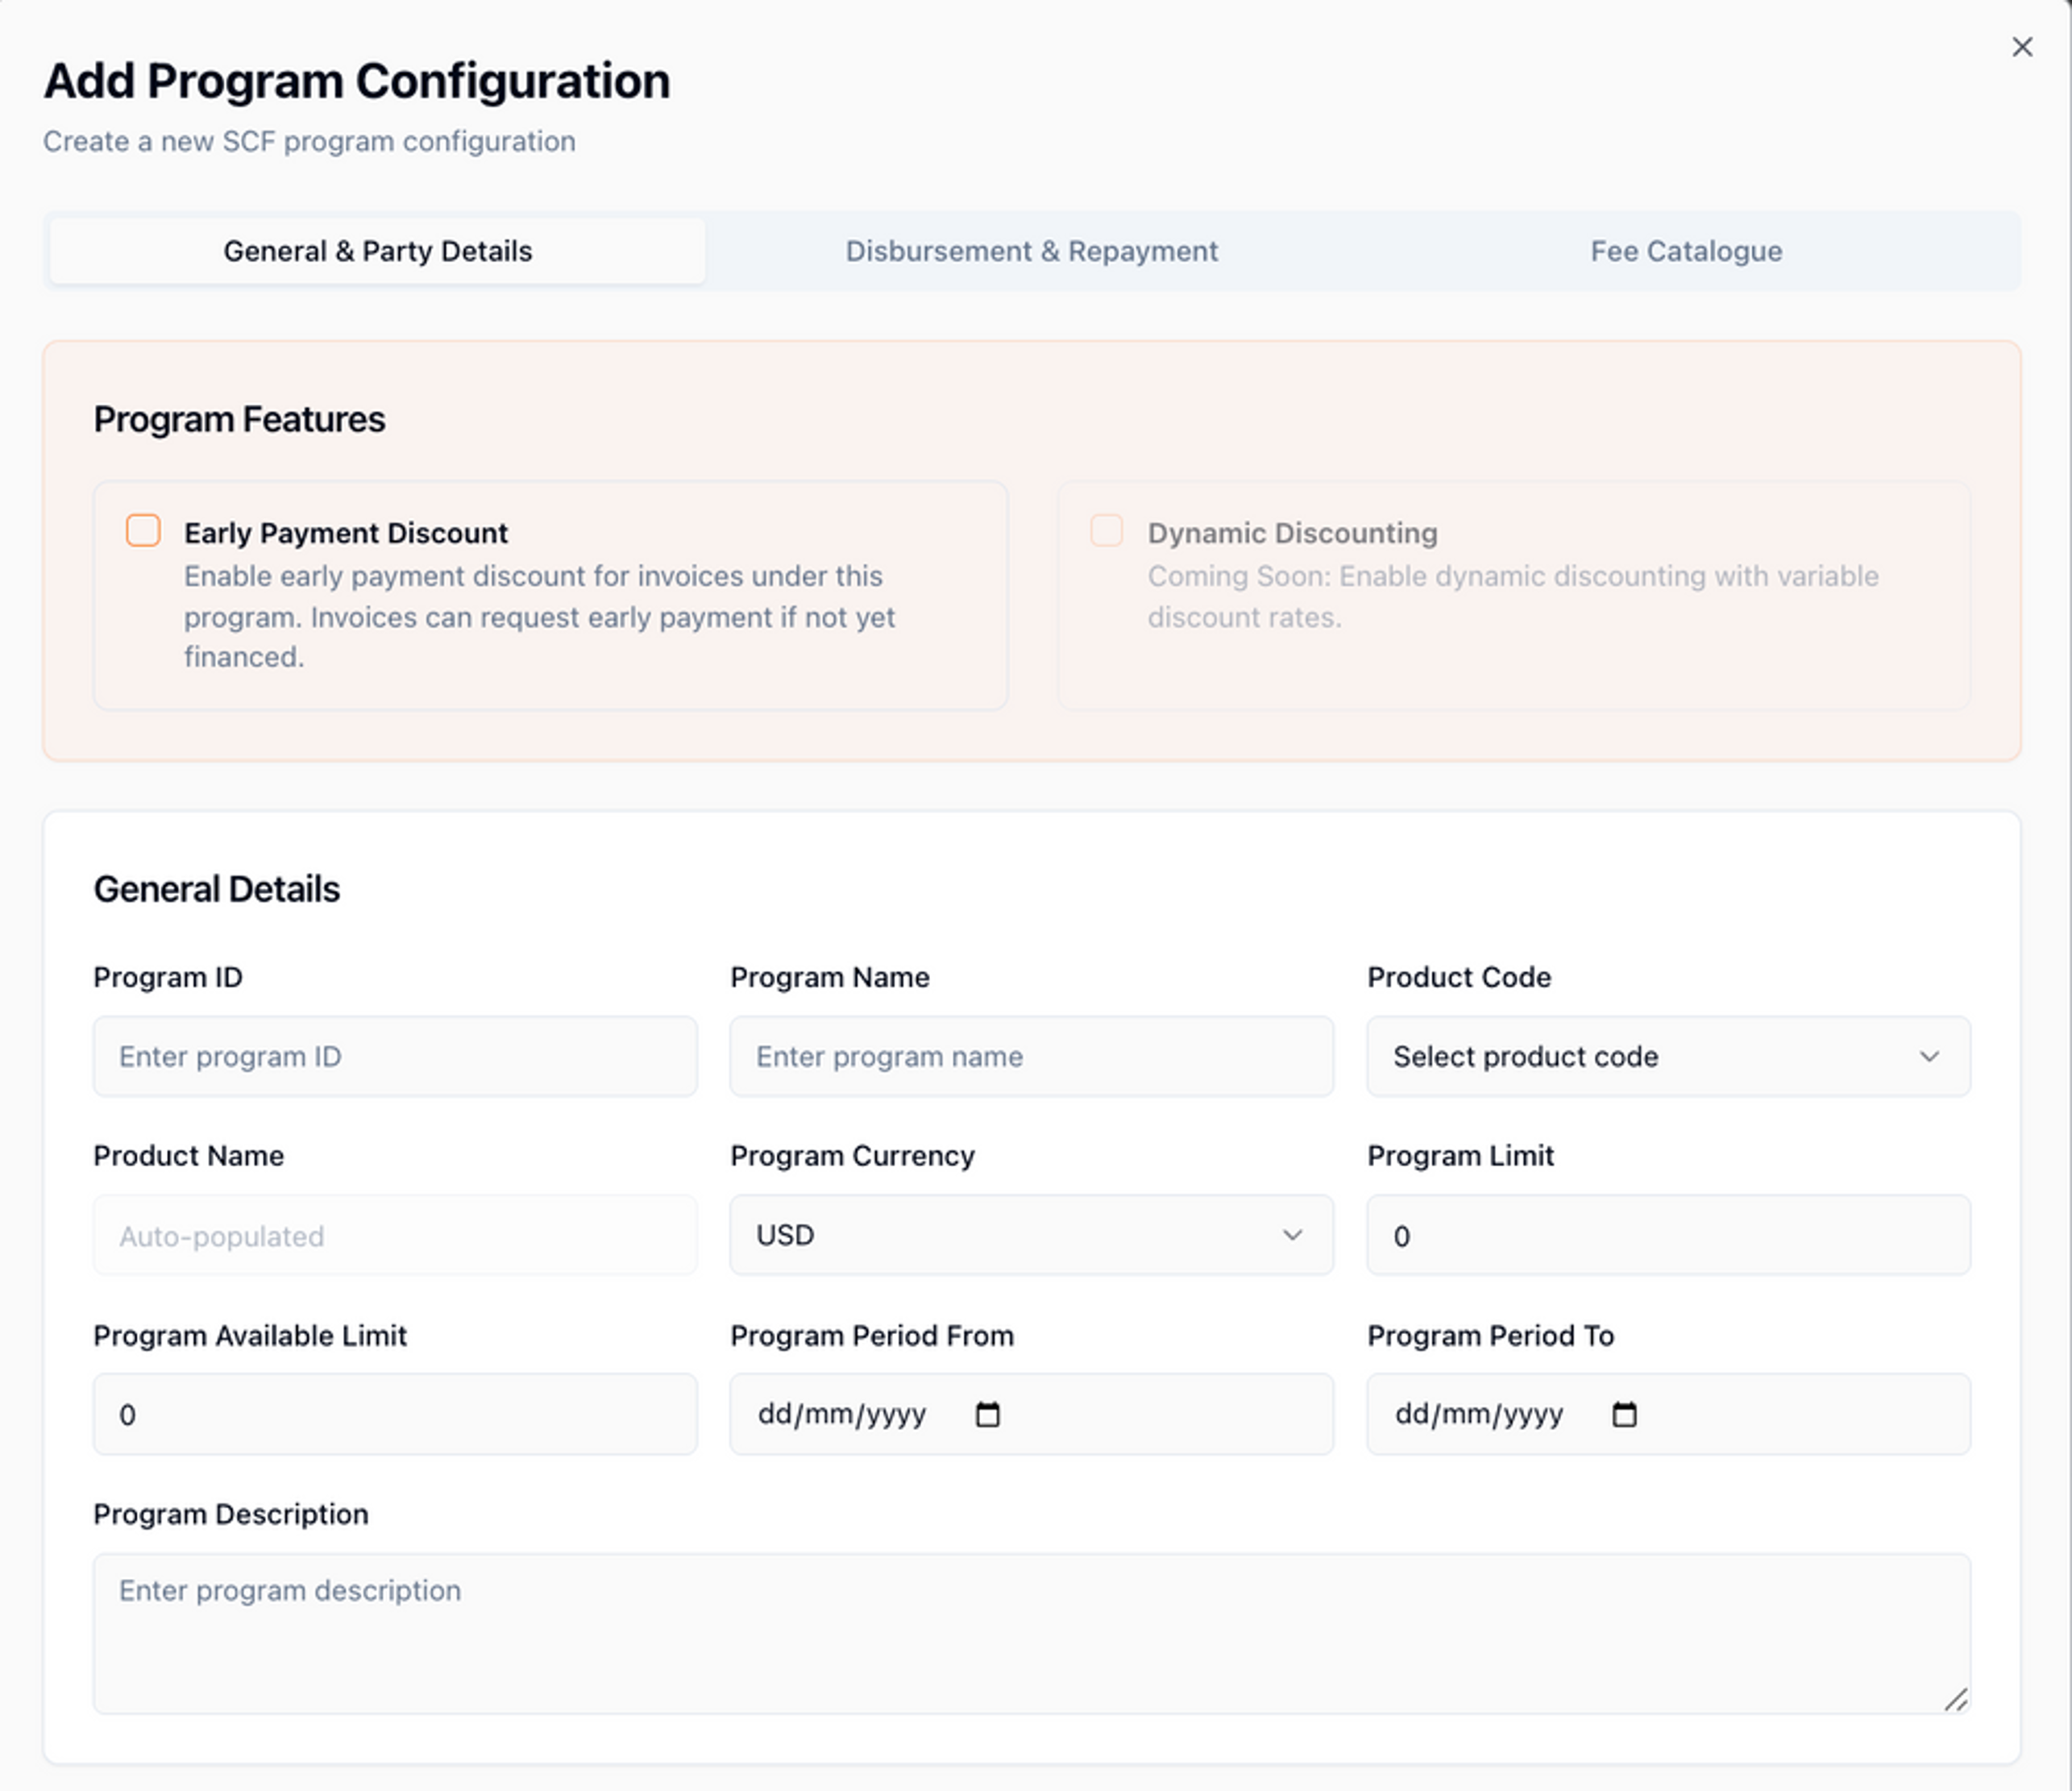
\includegraphics[width=\textwidth, keepaspectratio]{images/platform_program_creation_form.png}
    \caption{Program configuration creation form}
    \label{fig:ch4_program_creation_form}
\end{figure}

\subsection{Counterparty Onboarding and Foundational Data}
\label{subsec:counterparty_foundational_ui}

\texttt{SCFCounterPartyOnboarding} provides table-based management of counterparties, inline creation and editing, document upload, maker/checker actions, bulk creation, and CSV export. The component is connected to backend operations through \texttt{scfCounterPartyService}.

[Insert screenshot of Counterparty Onboarding table and actions]

Foundational data screens such as \texttt{CityMaster}, \texttt{CountryMaster}, \texttt{CurrencyMaster}, and \texttt{StateMaster} provide CRUD interfaces for reference values. These screens may appear less complex than program configuration, but they support the integrity of the wider system. A program or counterparty form depends on stable reference data.

\subsection{Control Centre}
\label{subsec:control_centre}

The control centre groups configurable UI and field behavior modules. \texttt{FieldDefinition} manages custom field definitions. \texttt{FieldActionsTab} configures action rules at field level. \texttt{ManagePanesAndSections} handles layout configuration. \texttt{ProductEventMapping} connects product events to platform behavior. These modules show that the frontend is not only a static set of forms; part of its purpose is to expose controlled configuration surfaces to bank administrators.

\section{Invoice Management Flows}
\label{sec:invoice_management_flows}

\subsection{Invoice Upload Flow}
\label{subsec:invoice_upload_flow}

Invoice upload is orchestrated by \texttt{InvoiceUploadForm}. The component coordinates the Excel uploader, scanned invoice uploader, validation table, summary cards, disbursement eligibility display, rejection report download, progress state, and error display. Figure~\ref{fig:ch4_invoice_upload_flow} summarizes the component flow.

\begin{figure}[H]
    \centering
    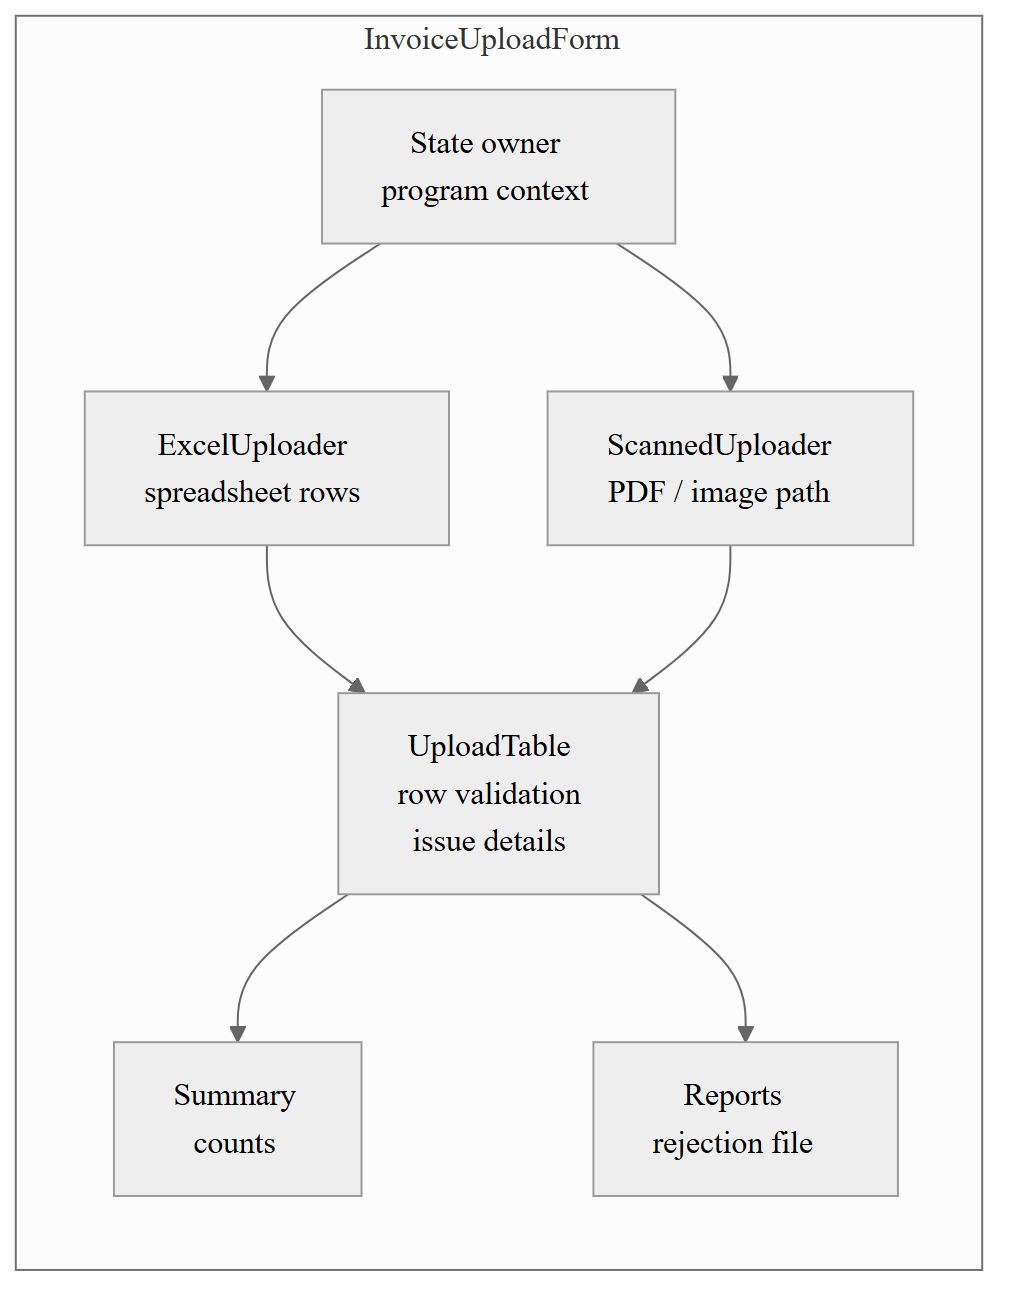
\includegraphics[width=\textwidth, keepaspectratio]{diagram_as_code/images/png/ch4_invoice_upload_flow.png}
    \caption{Invoice upload component flow}
    \label{fig:ch4_invoice_upload_flow}
\end{figure}

The Excel path uses \texttt{ExcelInvoiceUploader} for spreadsheet files. The scanned path uses \texttt{ScannedInvoiceUploader} for images or PDF files that may require OCR processing. Once uploaded, rows are displayed in \texttt{InvoiceUploadTable}, with validation status and row-level issues. \texttt{ValidationSummaryCard} then aggregates the result, while \texttt{DisbursementStatusCard} gives an eligibility-oriented view.

\begin{figure}[H]
    \centering
    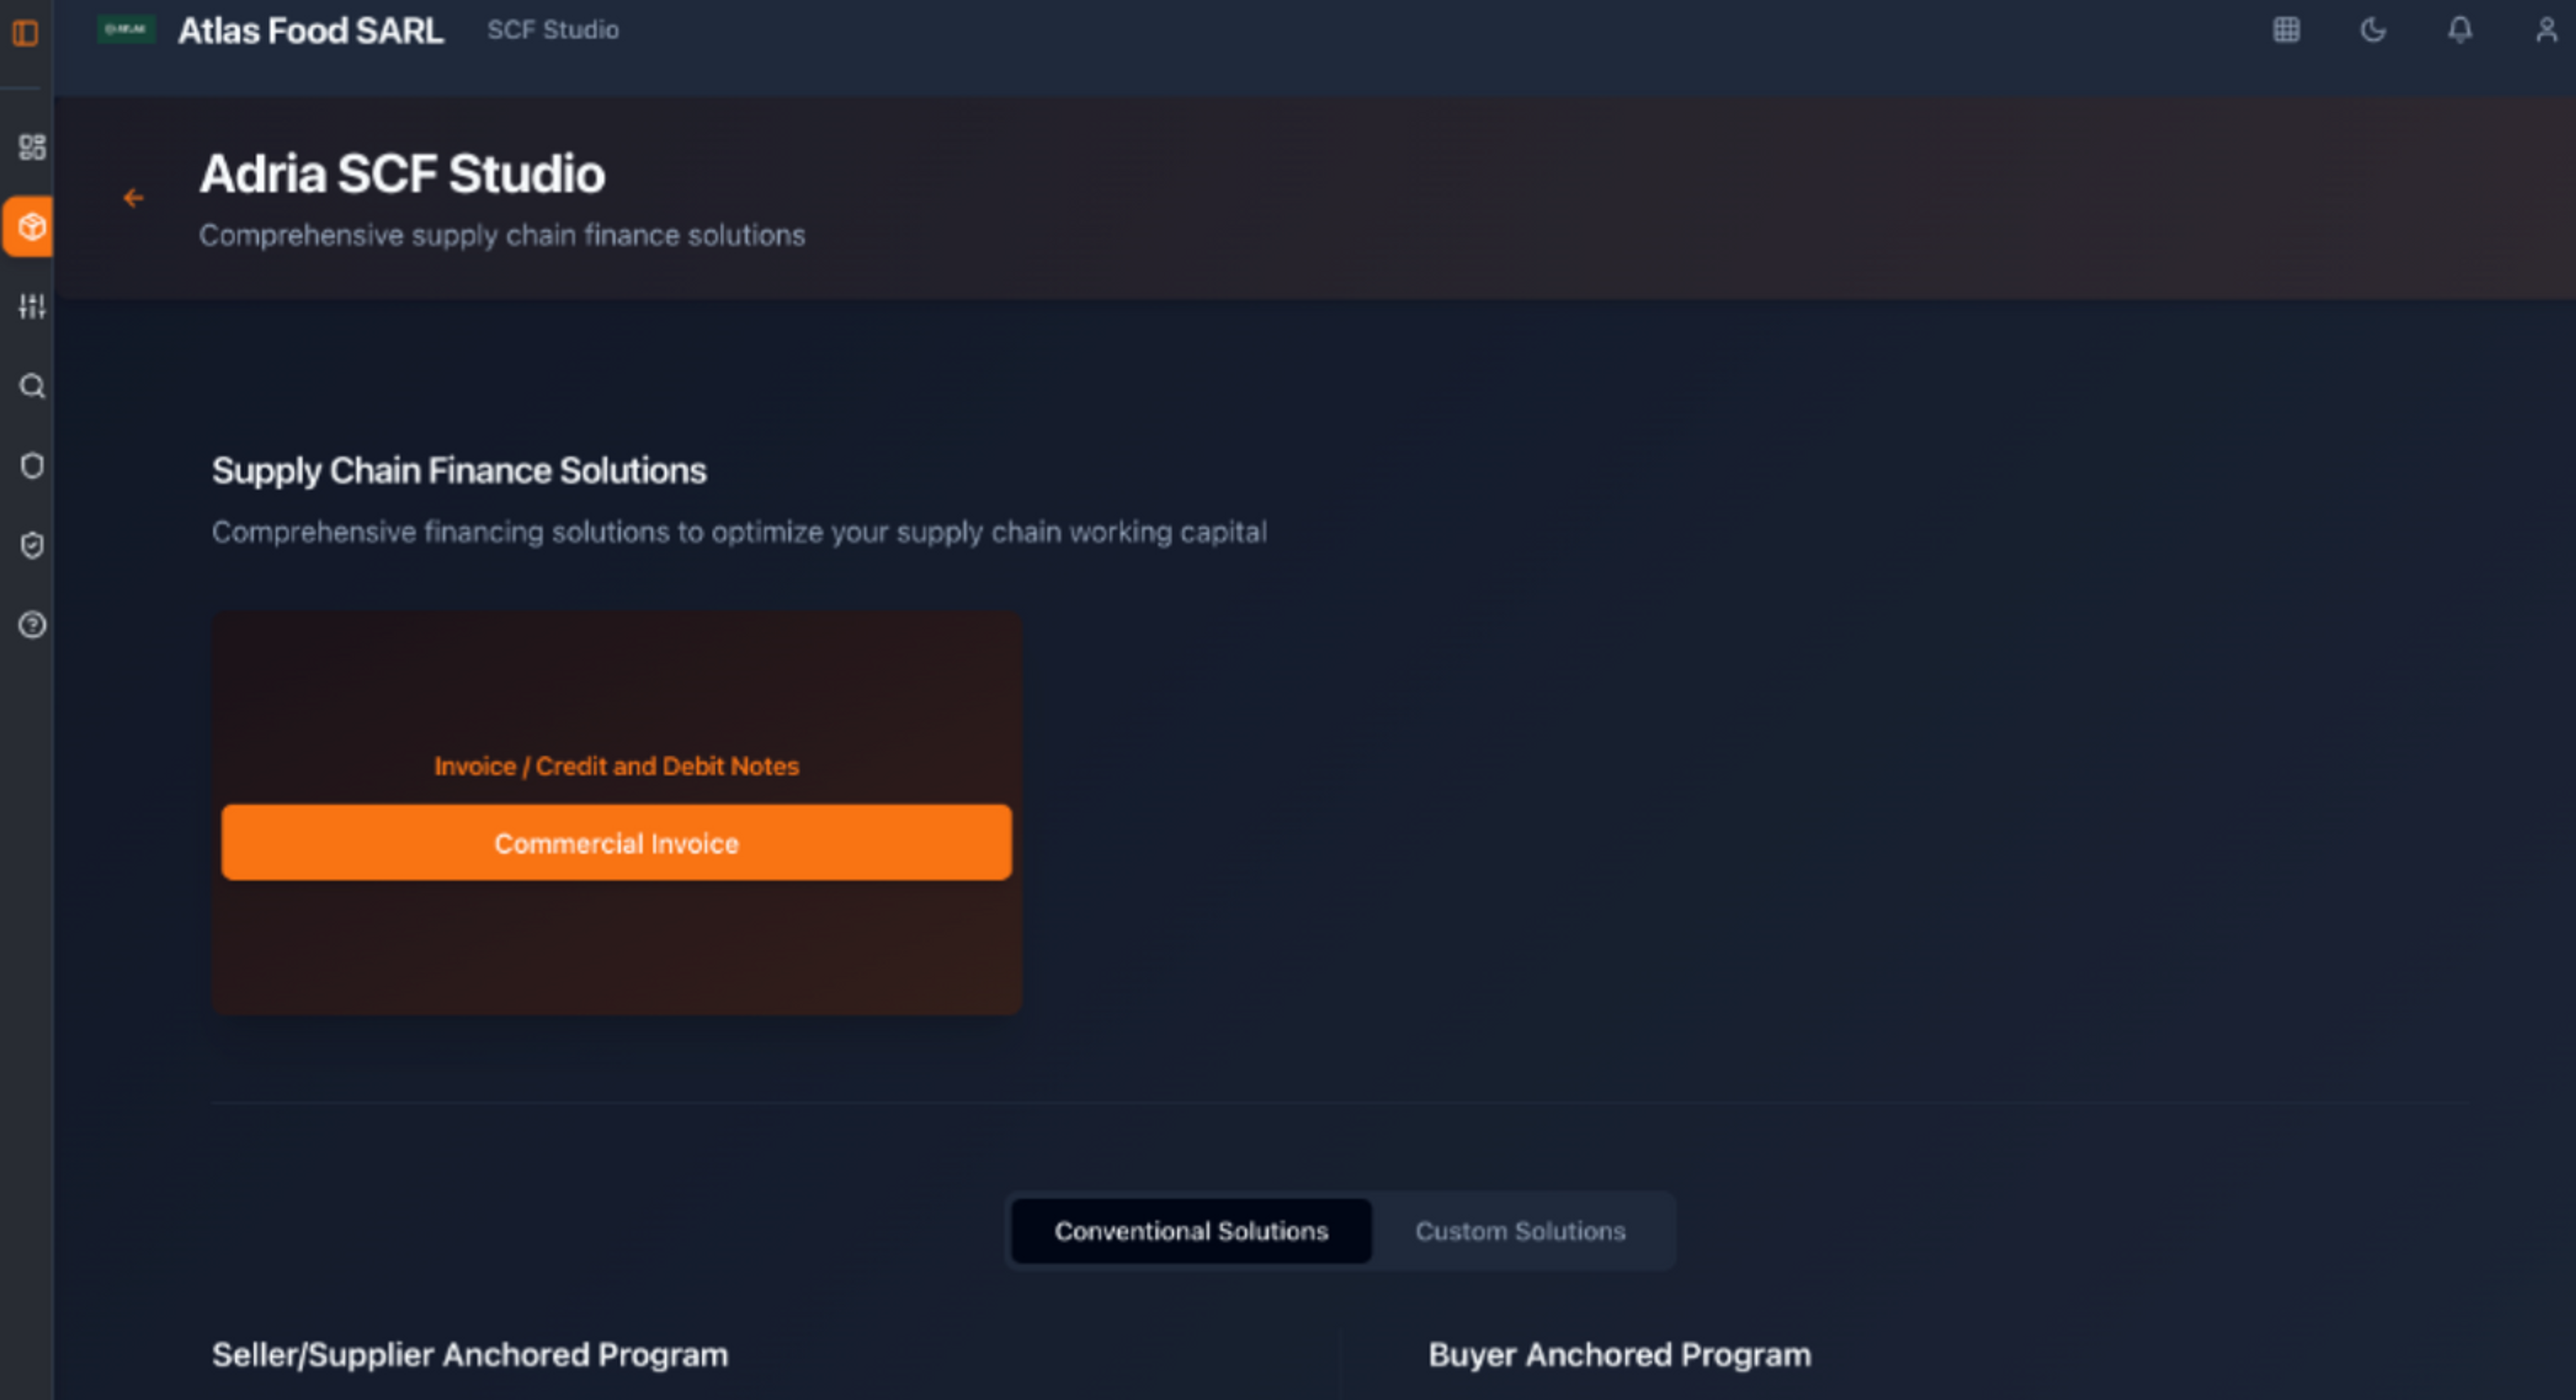
\includegraphics[width=\textwidth, keepaspectratio]{images/platform_invoice_creation_upload.png}
    \caption{Invoice management screen with upload processing method}
    \label{fig:ch4_invoice_creation_upload}
\end{figure}

\begin{figure}[H]
    \centering
    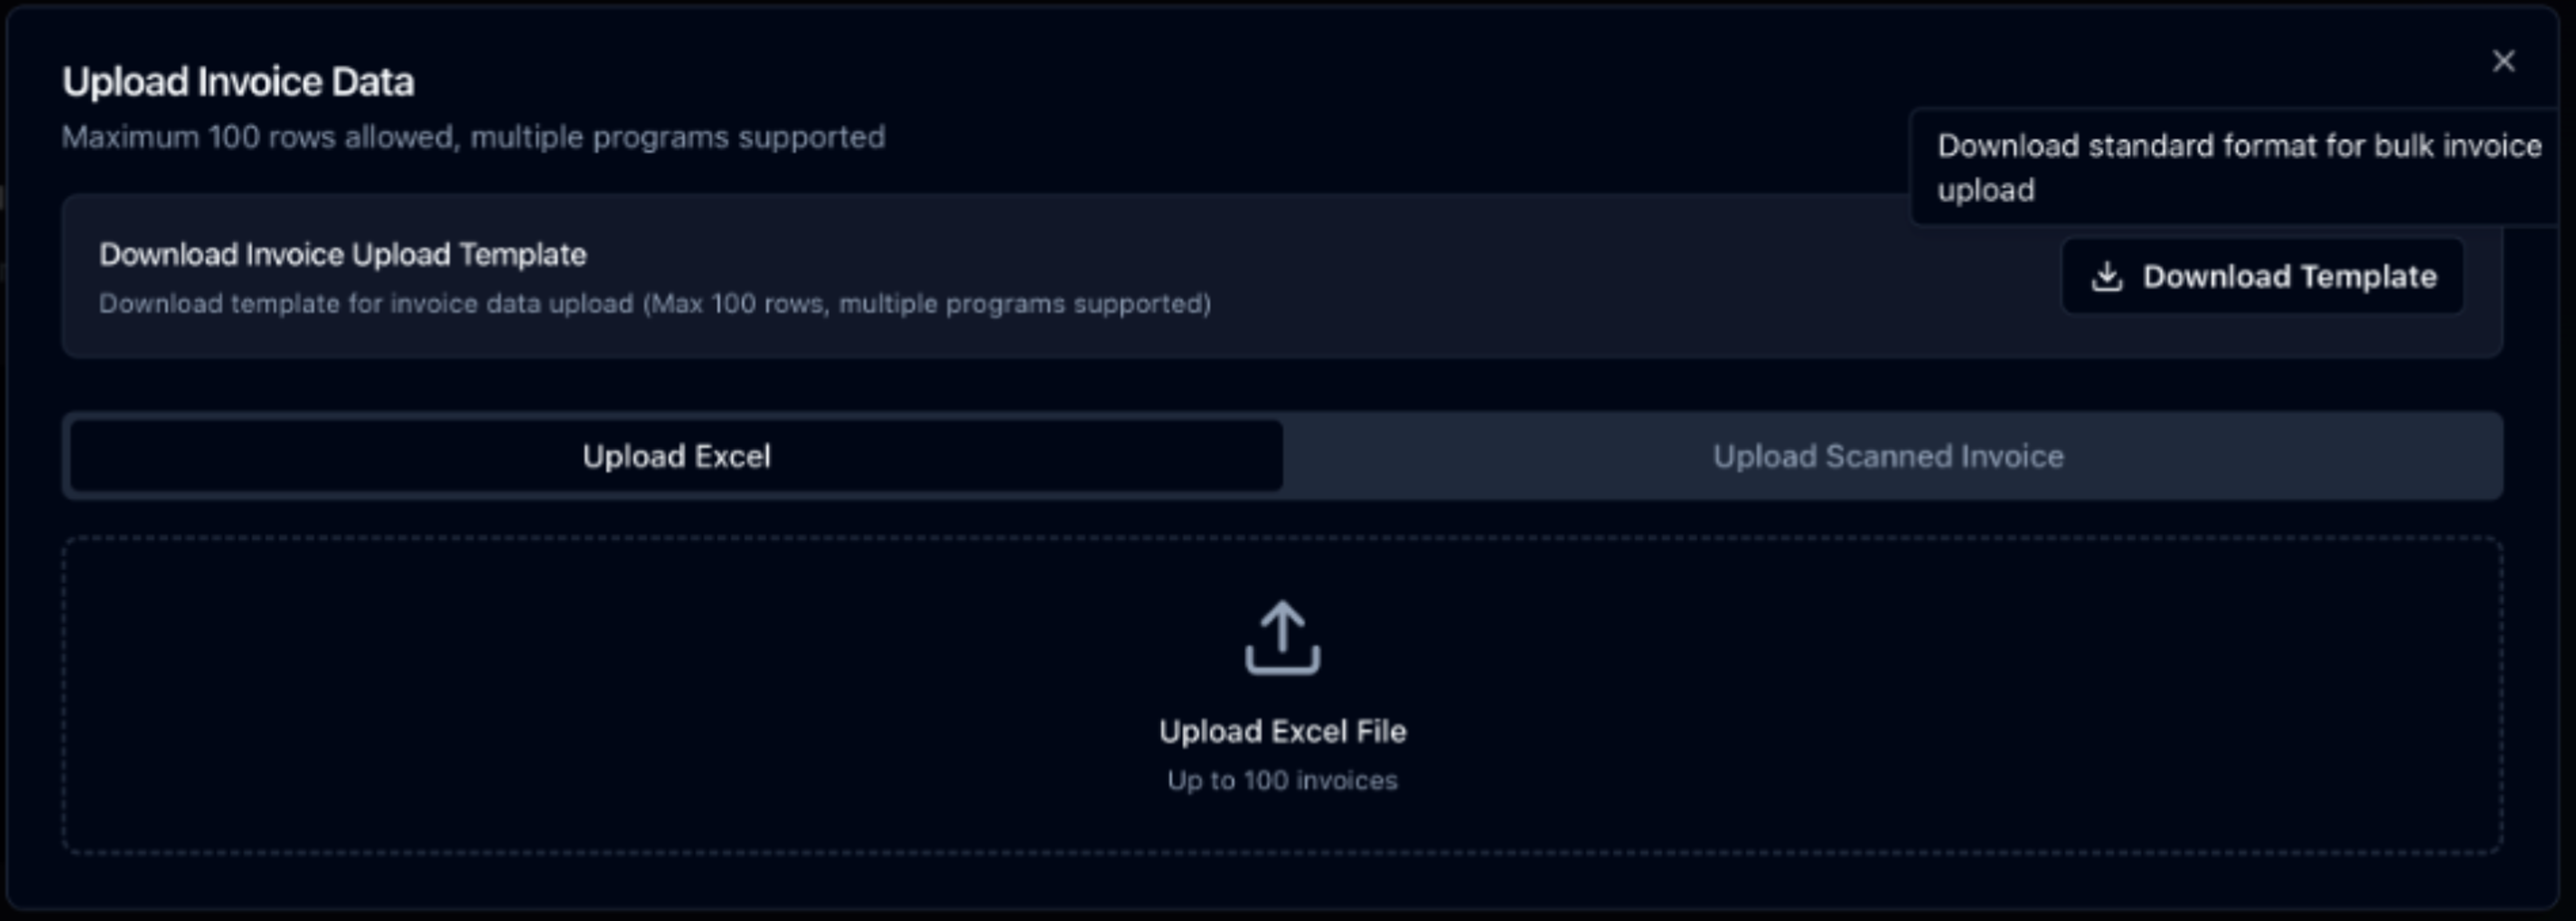
\includegraphics[width=\textwidth, keepaspectratio]{images/platform_invoice_upload.png}
    \caption{Invoice upload modal for Excel and scanned invoice files}
    \label{fig:ch4_invoice_upload_modal}
\end{figure}

\subsection{Manual Invoice Form}
\label{subsec:manual_invoice_form}

The manual invoice flow is handled by \texttt{InvoiceForm}. It is organized into panes: \texttt{InvoiceGeneralDetailsPane}, \texttt{InvoiceLineItemsPane}, and \texttt{InvoiceSummaryPane}. Supporting components such as \texttt{InvoiceProgressIndicator}, \texttt{InvoicePaneRenderer}, and \texttt{InvoiceFormActions} give structure to the form experience.

The \texttt{useInvoiceForm} hook centralizes state and calculation logic. This pattern keeps the panes focused on presentation and interaction rather than forcing each one to carry the whole form model. For multi-pane forms, that distinction helps readability.

\begin{figure}[H]
    \centering
    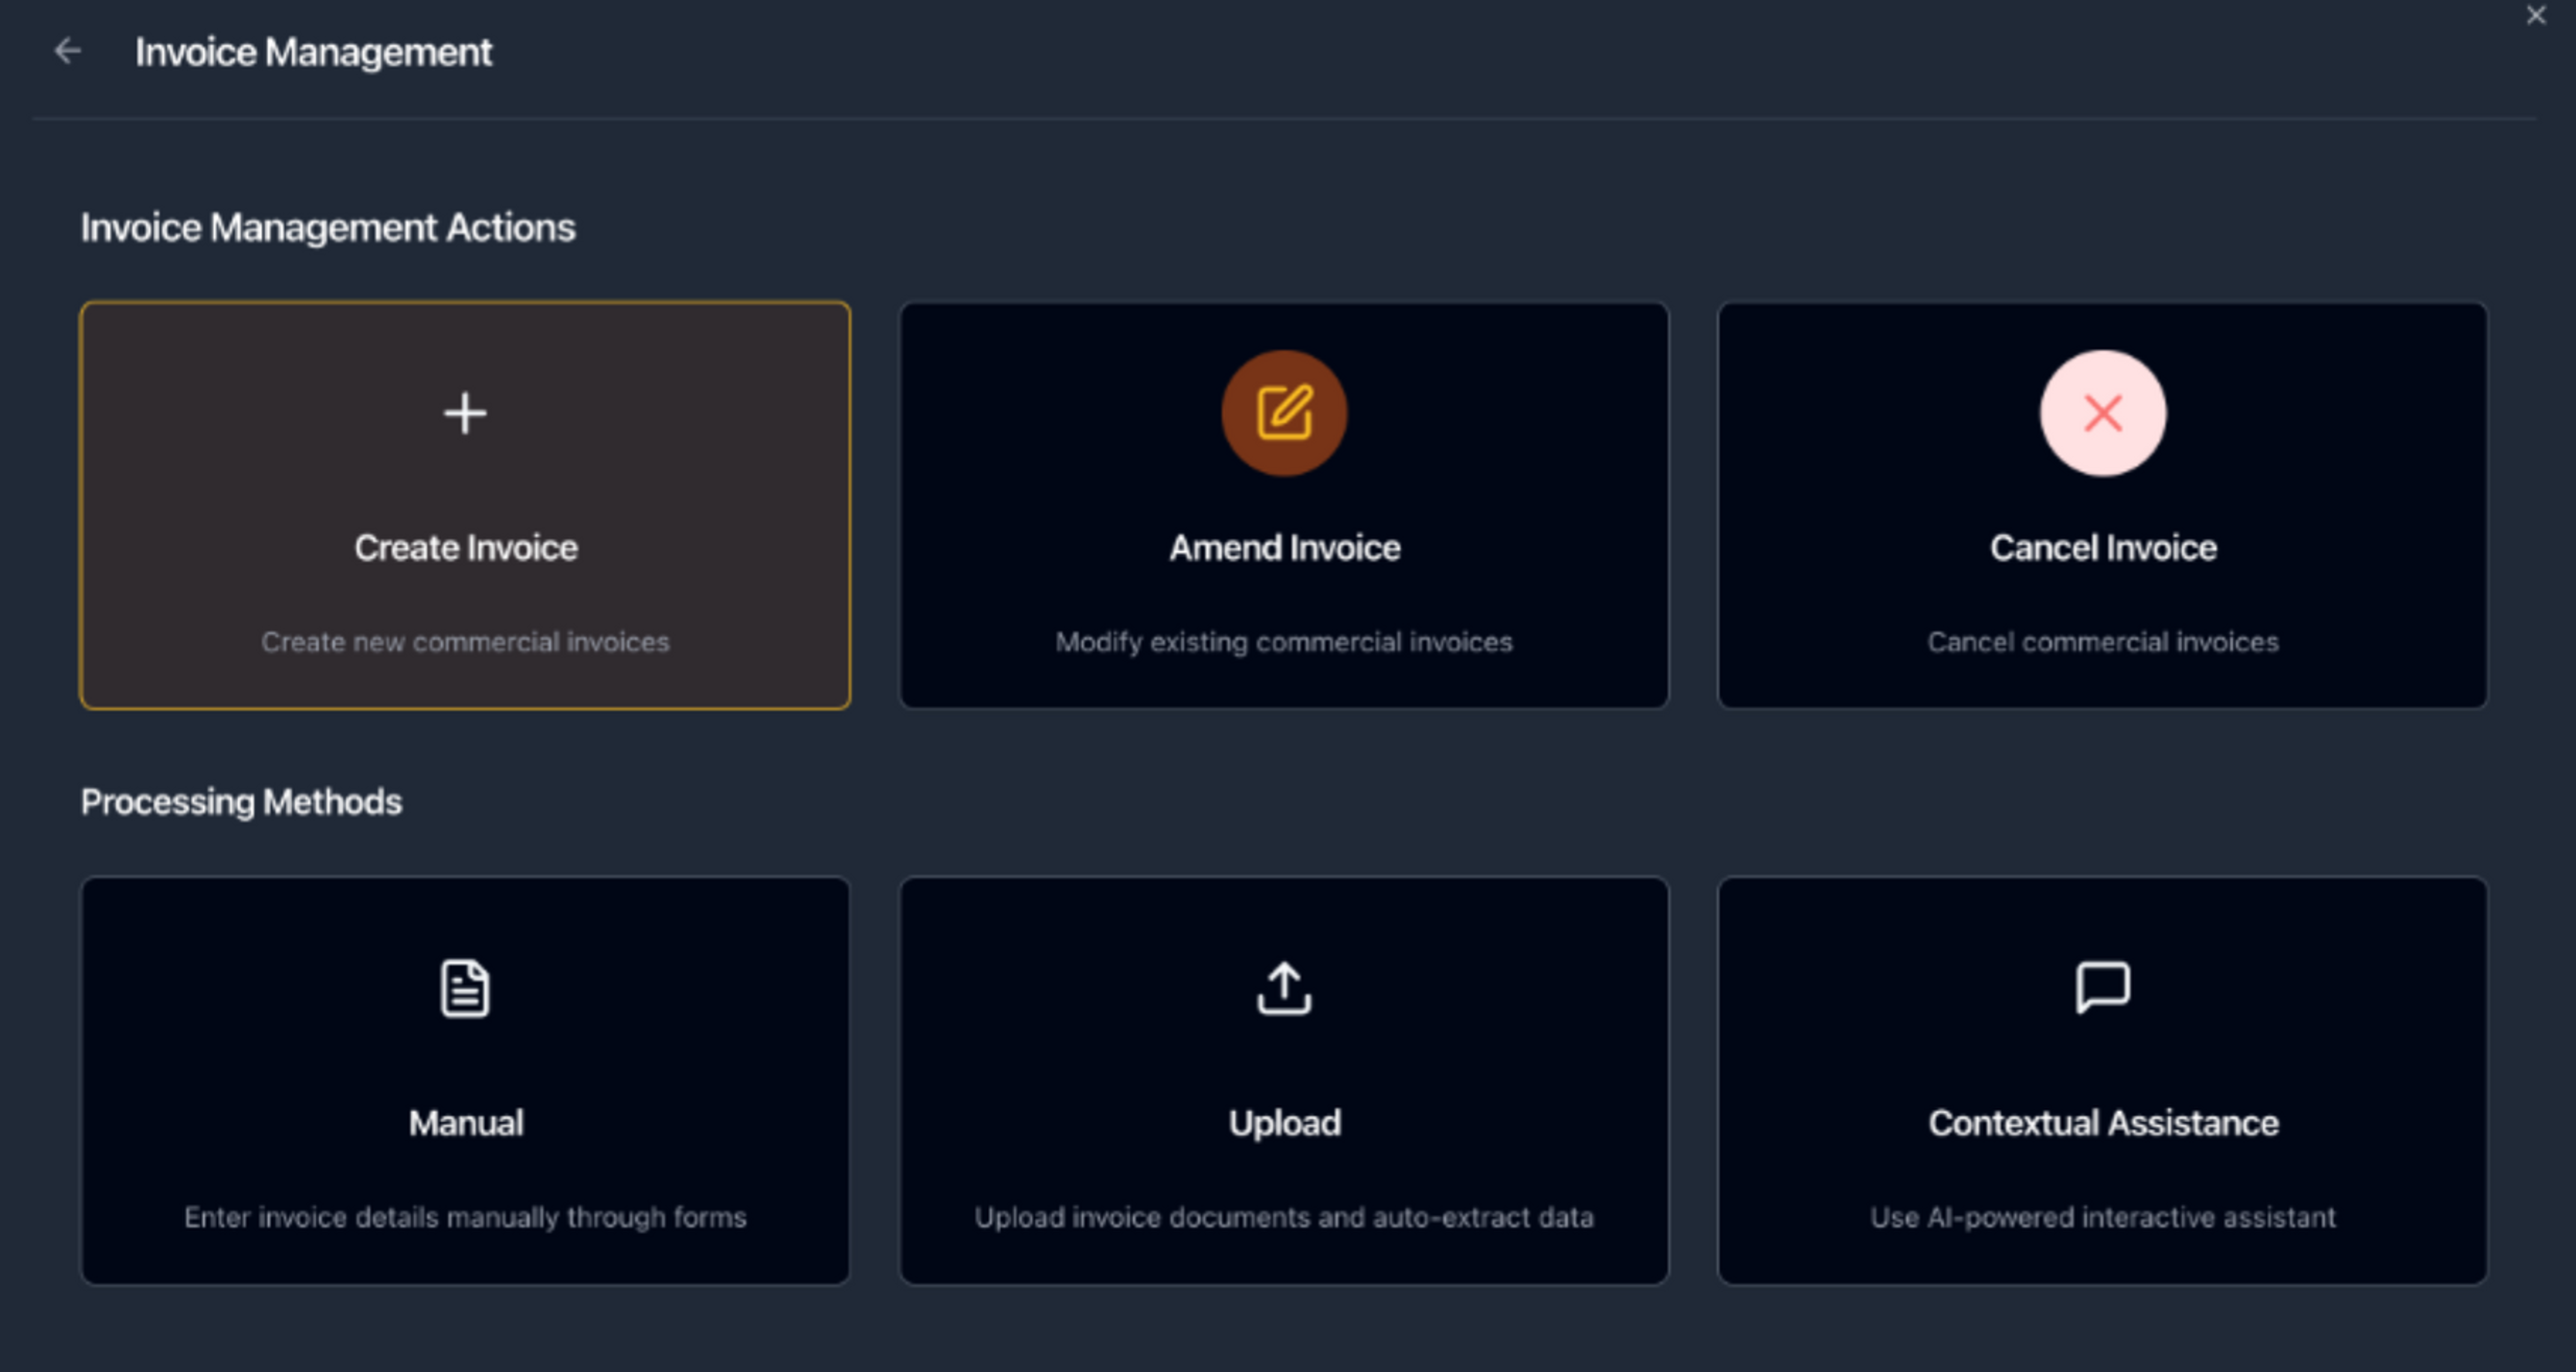
\includegraphics[width=\textwidth, keepaspectratio]{images/platform_invoice_creation_manual.png}
    \caption{Manual invoice creation entry point}
    \label{fig:ch4_invoice_creation_manual}
\end{figure}

\section{Finance and Early Payment Flows}
\label{sec:finance_early_payment}

\subsection{Early Payment Request}
\label{subsec:early_payment_request}

The early payment flow is implemented through \texttt{EarlyPaymentRequestModal} and \texttt{EarlyPaymentRequestForm}. It captures the requested payment date, whether the discount is accepted, and the calculated net amount. The operation connects to \texttt{earlyPaymentService}, which maps the frontend action to the backend endpoint.

This flow is smaller than the disbursement wizard, but it is highly meaningful in SCF. Early payment is one of the places where a commercial obligation becomes a financing decision, and the interface must make timing, discount, and acceptance clear to the user.

\subsection{Finance Disbursement Wizard}
\label{subsec:finance_disbursement_wizard}

The finance disbursement flow is implemented as a six-step wizard inside \texttt{FinanceDisbursementModal}. The panes are \texttt{ProgramProductSelectionPane}, \texttt{InvoiceSelectionPane}, \texttt{FinanceDetailsPane}, \texttt{RepaymentDetailsPane}, \texttt{AccountingEntriesPane}, and \texttt{ReviewSubmitPane}. Figure~\ref{fig:ch4_finance_disbursement_wizard} presents the corrected wizard order, while Figure~\ref{fig:ch4_manual_disbursement_screen} shows the current platform screen.

\begin{figure}[H]
    \centering
    
\includegraphics[width=\textwidth, keepaspectratio]{images/ch4_finance_disbursement_wizard.png}
    \caption{Finance disbursement six-step wizard}
    \label{fig:ch4_finance_disbursement_wizard}
\end{figure}

The first pane selects the program and product context. The invoice pane loads eligible invoices and allows the user to select which invoices will be financed. The finance details pane captures terms and presents fee breakdown information. The repayment pane configures schedule-related details. Accounting entries are displayed as debit and credit lines before the final review. The final pane reviews the full request before submission.

\begin{figure}[H]
    \centering
    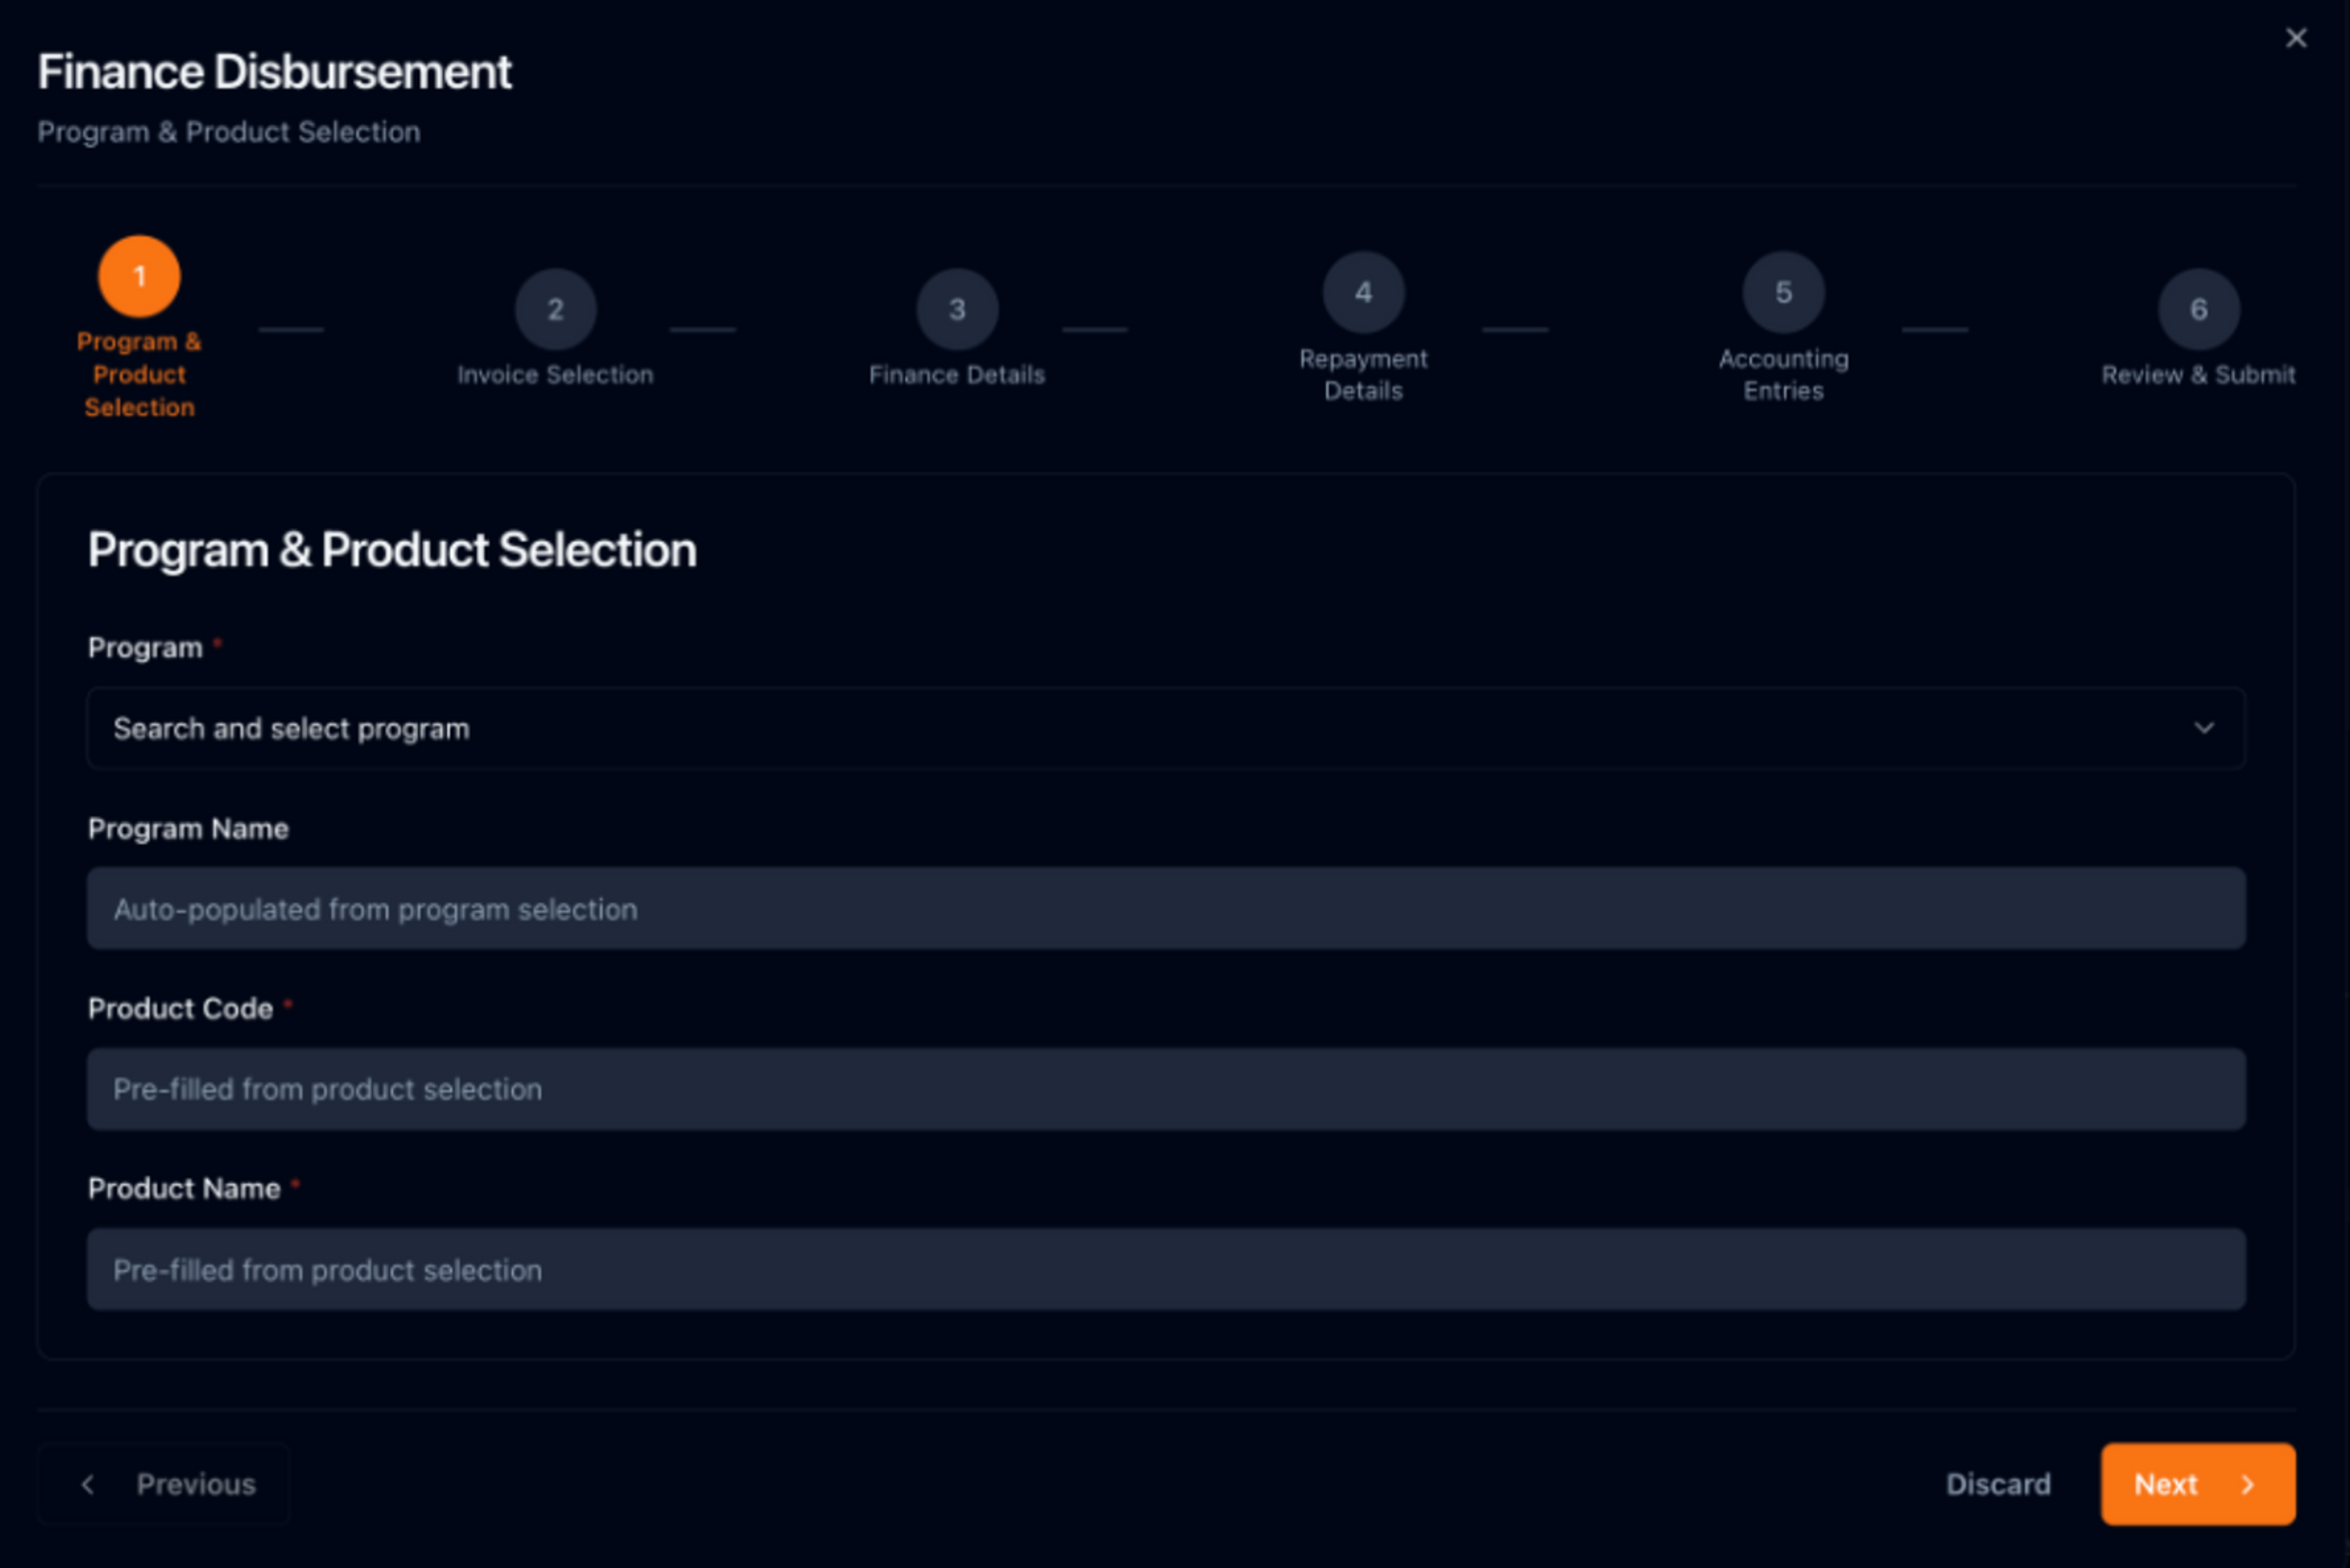
\includegraphics[width=\textwidth, keepaspectratio]{images/platform_manual_disbursement.png}
    \caption{Manual finance disbursement wizard}
    \label{fig:ch4_manual_disbursement_screen}
\end{figure}

\section{Document Inquiry and Specification Documents}
\label{sec:document_inquiry_specification}

\texttt{DocumentInquiry} gives users a filtered browsing interface for documents. \texttt{DocumentUploadPopup} handles file selection and upload behavior, while \texttt{DocumentUploadDetails} supports viewing and downloading. The same document concerns described in earlier chapters reappear here in interface form: the user does not see MinIO or presigned URL generation directly, but the UI must expose a smooth document lifecycle.

The \texttt{SpecificationDocument} page is routed separately and protected through \texttt{AuthGuard}. It provides a dedicated surface for specification-related documents, which is useful in a platform where functional rules, API specifications, and operational references may evolve alongside development.

\section{Notifications Panel}
\label{sec:notifications_panel}

\texttt{NotificationsPanel} provides a place for user-facing events and alerts. Although the current context does not describe a complete notification backend, the component is part of the frontend structure. In an SCF platform, notifications naturally belong near approval events, validation outcomes, document status changes, and financing decisions.

\section{Forms Engineering: Patterns and Practices}
\label{sec:forms_engineering}

\subsection{Hooks and Form State}
\label{subsec:hooks_form_state}

Several frontend flows are too large to be kept inside a single component without becoming fragile. The project uses custom hooks such as \texttt{useInvoiceForm}, \texttt{useProgramForm}, \texttt{useBusinessView}, \texttt{useAuth}, and \texttt{useFieldActions}. These hooks separate reusable behavior from visual components.

\subsection{Error Handling and User Feedback}
\label{subsec:error_feedback}

The application includes Sonner-based toast feedback through the global \texttt{Toaster}. API errors are supported by helper logic such as \texttt{scfApiError.ts}. This matters because banking forms are validation-heavy. A failed upload, a rejected field, or an expired token should not leave the user guessing.

\section{API Services Layer}
\label{sec:api_services_layer}

\subsection{Axios Client and Endpoint Mapping}
\label{subsec:axios_endpoint_mapping}

The shared Axios client is defined under \texttt{integrations/gateway/client.ts}. It reads the access token from session storage and attaches it as a bearer token. On unauthorized responses, it attempts refresh behavior and logs the user out if the session cannot be recovered.

Feature services wrap this client with typed functions. Examples include \texttt{scfProgramConfigService}, \texttt{scfProductService}, \texttt{invoiceUploadService}, \texttt{financeDisbursementService}, \texttt{documentInquiryService}, and foundational data services. Figure~\ref{fig:ch4_services_layer} shows this layering.

\begin{figure}[H]
    \centering
    
\includegraphics[width=\textwidth, keepaspectratio]{images/ch4_services_layer.png}
    \caption{Frontend services layer}
    \label{fig:ch4_services_layer}
\end{figure}

\subsection{TypeScript Types}
\label{subsec:typescript_types}

The frontend model is supported by TypeScript type files. \texttt{invoiceUpload.ts} defines upload files, upload rows, validation statuses, upload results, and disbursement eligibility. \texttt{scfTransaction.ts} defines transaction records, finance disbursement details, fee breakdowns, accounting entries, repayment entries, and approval history.

\begin{table}[H]
    \centering
    \caption{Frontend implementation patterns}
    \label{tab:ch4_frontend_patterns}
    \standardtable
    \begin{tabularx}{\textwidth}{B{0.28\textwidth} Y}
        \standardtablehead{\textbf{Pattern} & \textbf{Role in the frontend}}
        Protected route & Ensures that sensitive pages are rendered only for authenticated users. \\
        Business view hook & Converts Keycloak roles into BANK, ANCHOR, or COUNTERPARTY interface behavior. \\
        Feature service & Encapsulates gateway endpoint calls behind typed frontend functions. \\
        Wizard panes & Breaks long banking workflows into ordered, reviewable steps. \\
        TypeScript model & Documents the expected shape of invoices, transactions, disbursements, and validation results. \\
    \end{tabularx}
    \standardtableend
\end{table}

\section{Conclusion}
\label{sec:ch4_conclusion}

This chapter examined the frontend implementation of the SCF platform. The React application is structured around protected routing, Keycloak integration, role-based navigation, feature modules, custom hooks, typed services, and domain-specific forms. The frontend does not merely display backend data. It shapes the user's operational path through configuration, onboarding, invoice management, early payment, finance disbursement, transaction inquiry, and document handling.

The next chapter focuses on the Disbursement Module as the academic PFE project. It will connect the platform context, backend domain model, and frontend flows to the specific module assigned during the internship.
